\chapter{Conceptos}

\section{Conceptos Clave en la Lectura Profesional}

\subsection{Intenci\'on}

La \textbf{intenci\'on} se define como el prop\'osito oculto del operador profesional para influir en la direcci\'on del precio, manifest\'andose mediante patrones en volumen y velas. Se evidencia al observar:

\begin{itemize}
    \item Entrada relevante de volumen.
    \item Movimientos verticales y r\'apidos.
    \item Ruptura de zonas relevantes como rangos, soportes o resistencias y claviculares.
\end{itemize}

\begin{figure}[htb]
    \centering
    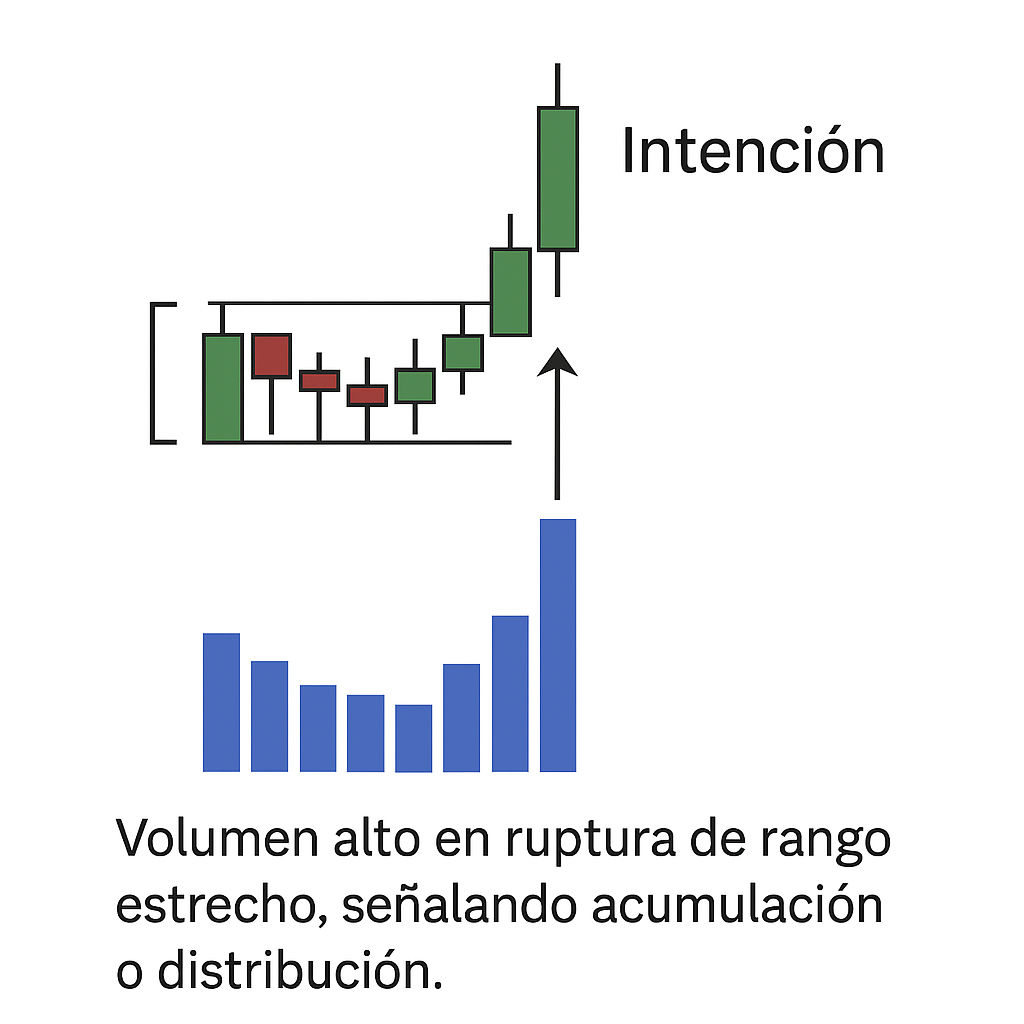
\includegraphics[width=11cm]{images/Intencion.png}
    \caption{Intenci\'on}
    \label{fig:Intencion}
\end{figure}

En la figura \ref{fig:Intencion} ...

\subsection{Desequilibrio}

El \textbf{desequilibrio} ocurre cuando una fuerza (oferta o demanda) domina claramente, impulsando movimientos significativos:

\begin{itemize}
    \item Se evidencia en velas amplias con alto volumen.
    \item Genera fases impulsivas como markup o markdown.
\end{itemize}

La combinaci\'on de estos elementos (intenci\'on, testeo y secado) facilita identificar momentos ideales para actuar en direcci\'on al desequilibrio.

\vspace{1em}
\noindent

\begin{figure}[!htbp]
    \centering
    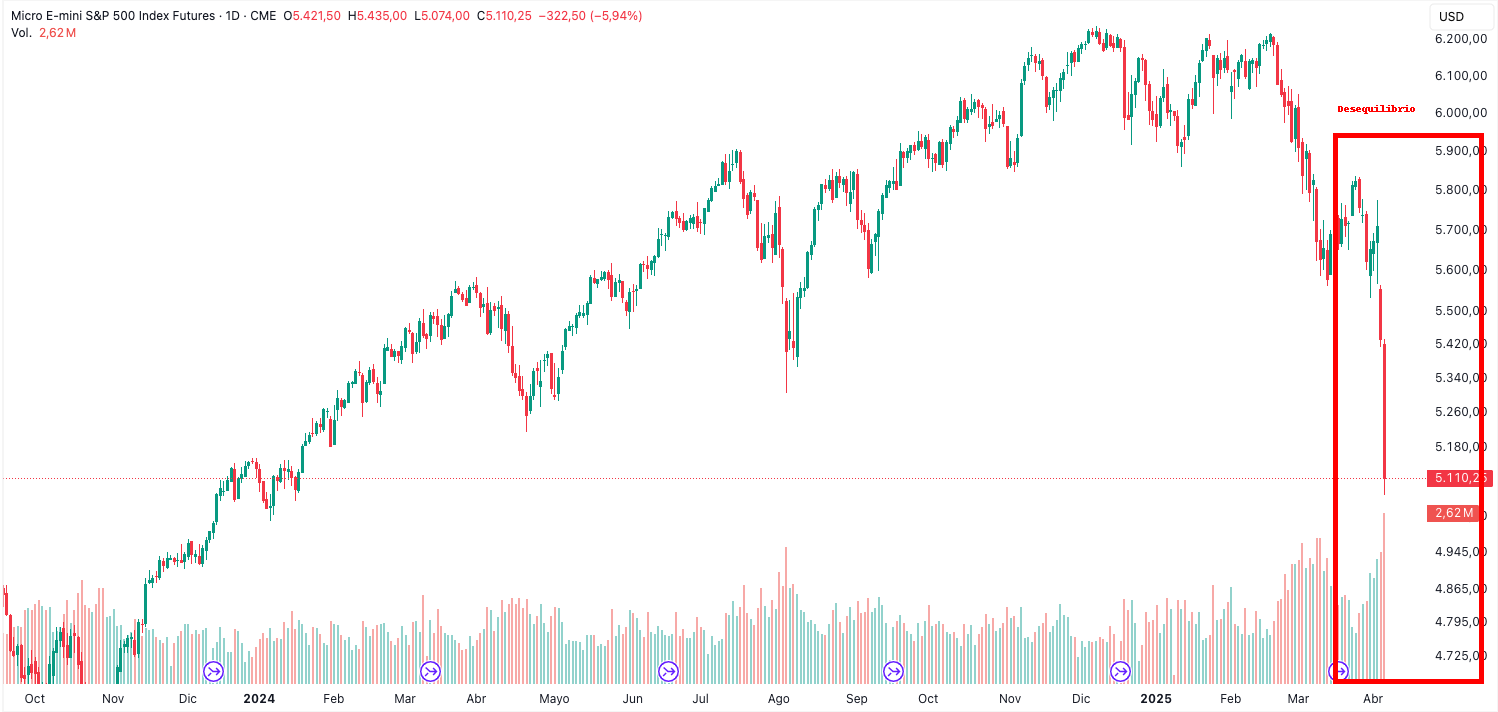
\includegraphics[width=11cm]{images/desequilibrio_mes0625_ampliado.png}
    \caption{Desequilibrio}
    \label{fig:desequilibrio_mes0625_ampliado}
\end{figure}
\vspace{0.5em}
\noindent

\subsection{Ejemplo de Desequilibrio en el MES-0625 (Abril 2025)}

En el contrato \textbf{MES-0625}, en el marco diario correspondiente al 4 de abril de 2025, figura \ref{fig:desequilibrio_mes0625_ampliado}, se observa un claro ejemplo de \textbf{desequilibrio bajista}:

\begin{itemize}
    \item El precio presenta una \textbf{vela bajista de cuerpo amplio}, con un rango significativamente mayor al promedio reciente.
    \item Esta vela rompe m\'ultiples soportes anteriores, generando una fase impulsiva tipo \textit{markdown}.
    \item El volumen asociado es el m\'as alto del per\'iodo observado, alcanzando los \textbf{2{,}62 millones de contratos}, lo cual confirma \textbf{intenci\'on profesional} en la acci\'on vendedora.
\end{itemize}

La combinaci\'on de una vela de amplio rango con volumen extremo constituye una manifestaci\'on clara de desequilibrio, validando la dominancia de la oferta en ese tramo del mercado.


\subsection{Secado}

El \textbf{secado} refleja la retirada deliberada de una de las partes profesionales del mercado:

\begin{itemize}
    \item Se caracteriza por un volumen muy bajo posterior a un movimiento.
    \item Suele preceder o formar parte del testeo.
    \item Indica ausencia de presi\'on contraria.
\end{itemize}

\begin{figure}[!htbp]
    \centering
    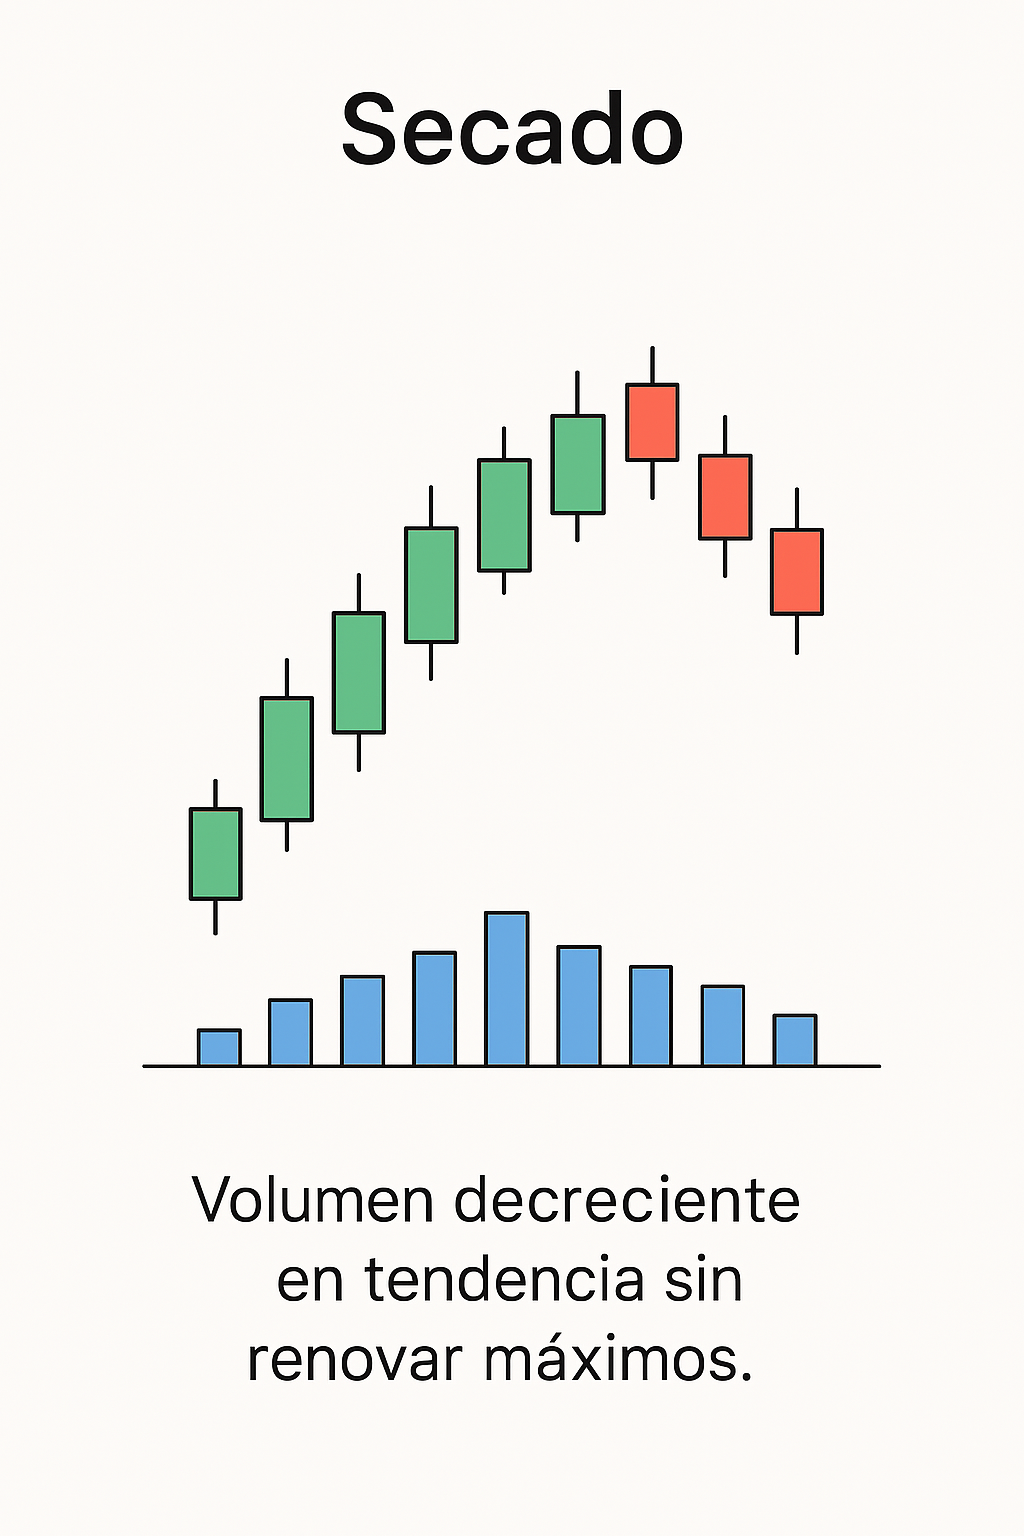
\includegraphics[width=11cm]{images/Secado.png}
    \caption{Secado}
    \label{fig:Secado}
\end{figure}

En la figura \ref{fig:Secado} ...

\subsection{Testeo}

El \textbf{testeo} es un movimiento correctivo con volumen estable o decreciente para evaluar si persiste presi\'on contraria tras una intenci\'on manifiesta:

\begin{itemize}
    \item No debe superar el origen del movimiento intencional previo.
    \item Si ocurre, debe recuperarse r\'apidamente.
\end{itemize}

\begin{figure}[!htbp]
    \centering
    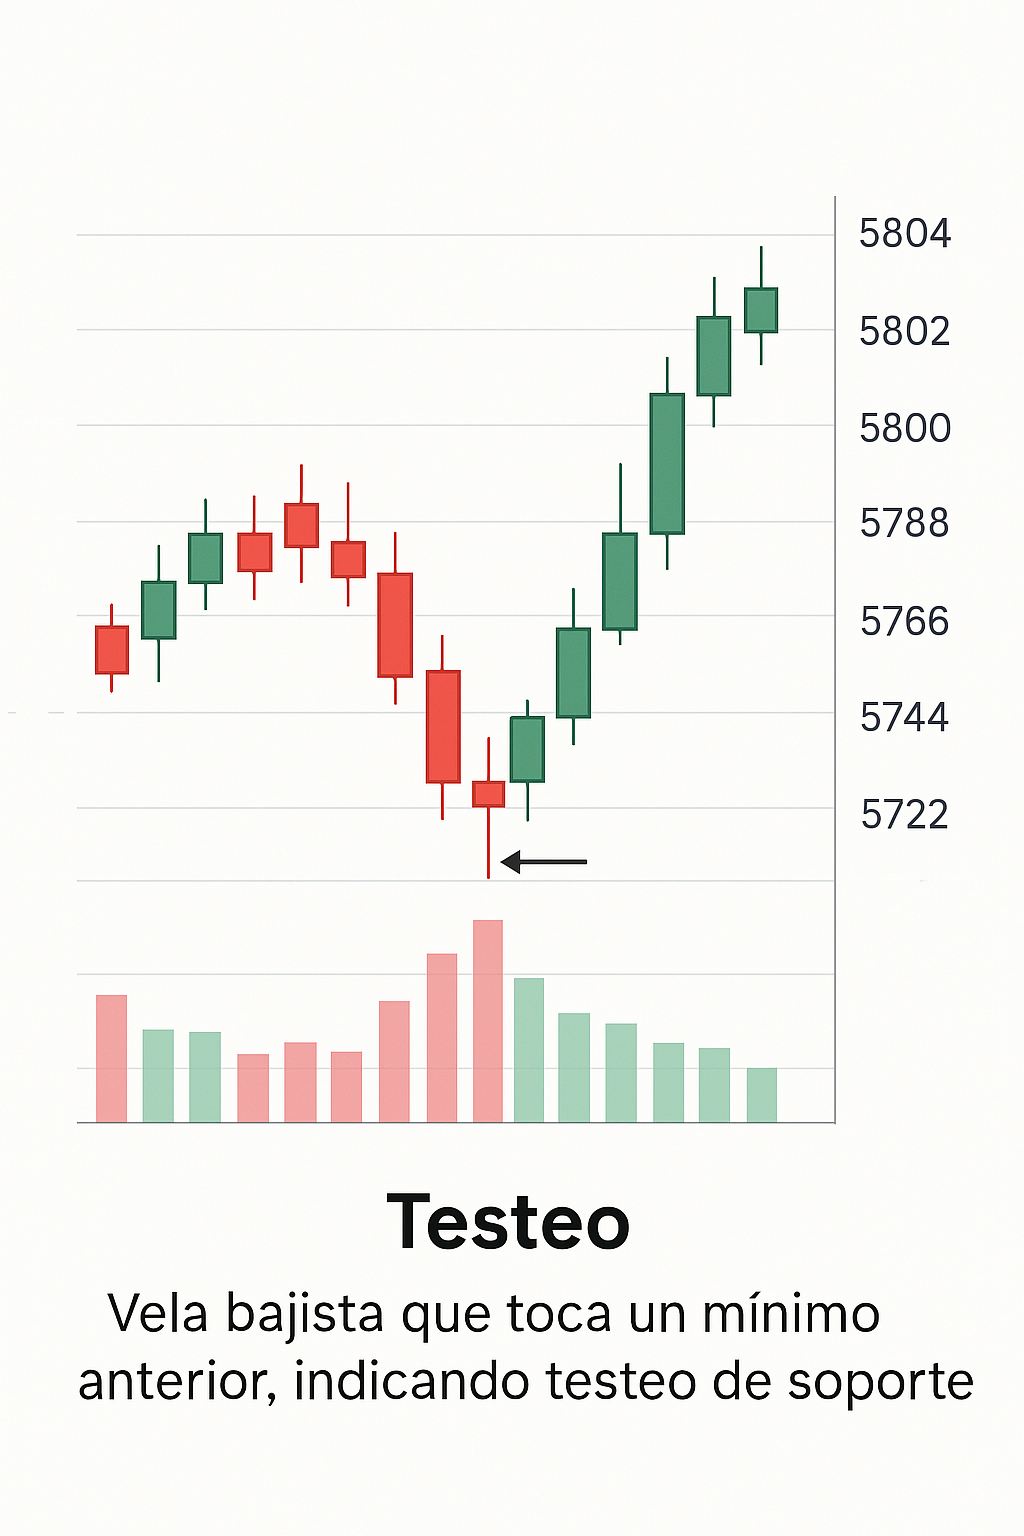
\includegraphics[width=11cm]{images/Testeo.png}
    \caption{Testeo}
    \label{fig:Testeo}
\end{figure}

En la figura \ref{fig:Testeo} ...

\subsection{Divergencia}

La \textbf{divergencia} se identifica por discordancias entre precio y volumen, indicando debilidad en la continuidad del movimiento:

\begin{itemize}
    \item Precio avanza, pero el volumen no lo respalda.
    \item Se busca en soportes, resistencias, directrices y zonas previamente operadas.
\end{itemize}

\begin{figure}[!htbp]
    \centering
    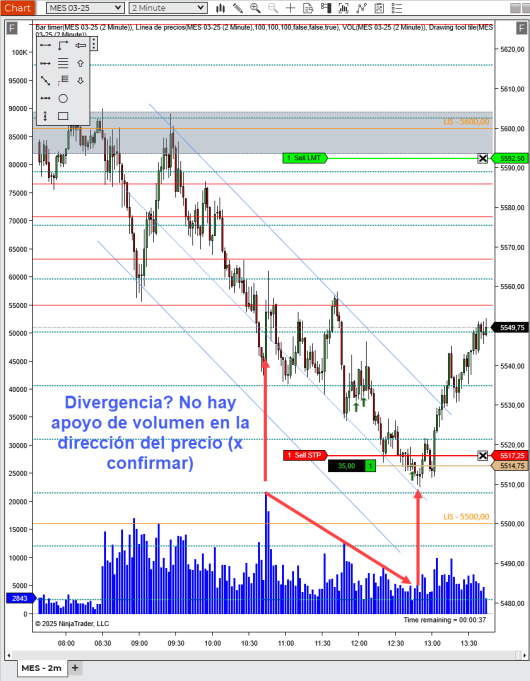
\includegraphics[width=11cm]{images/diver_1.png}
    \caption{Divergencia}
    \label{fig:diver_1}
\end{figure}

En la figura \ref{fig:diver_1} ...

\section{Fases y Estructuras del Profesional}

\subsection{Acumulaci\'on y Distribuci\'on}

\textbf{Acumulaci\'on}: compra institucional en un rango estrecho en la parte baja del gr\'afico.

\subsubsection*{Acumulaci\'on (Fase Profesional)}

\textbf{Descripci\'on textual:}

Proceso mediante el cual los operadores institucionales compran progresivamente en zonas de soporte, generalmente tras una fase de ca\'ida o correcci\'on prolongada. Se caracteriza por:

\begin{itemize}
    \item Movimiento lateral con m\'inimos similares.
    \item Volumen sostenido o creciente sin avance inmediato en el precio.
    \item Velas de rechazo alcista (\textit{pin bars}, \textit{engulfings}).
    \item Picos de volumen que coinciden con velas de rango estrecho o sombras inferiores largas.
\end{itemize}

\begin{figure}[!htbp]
    \centering
    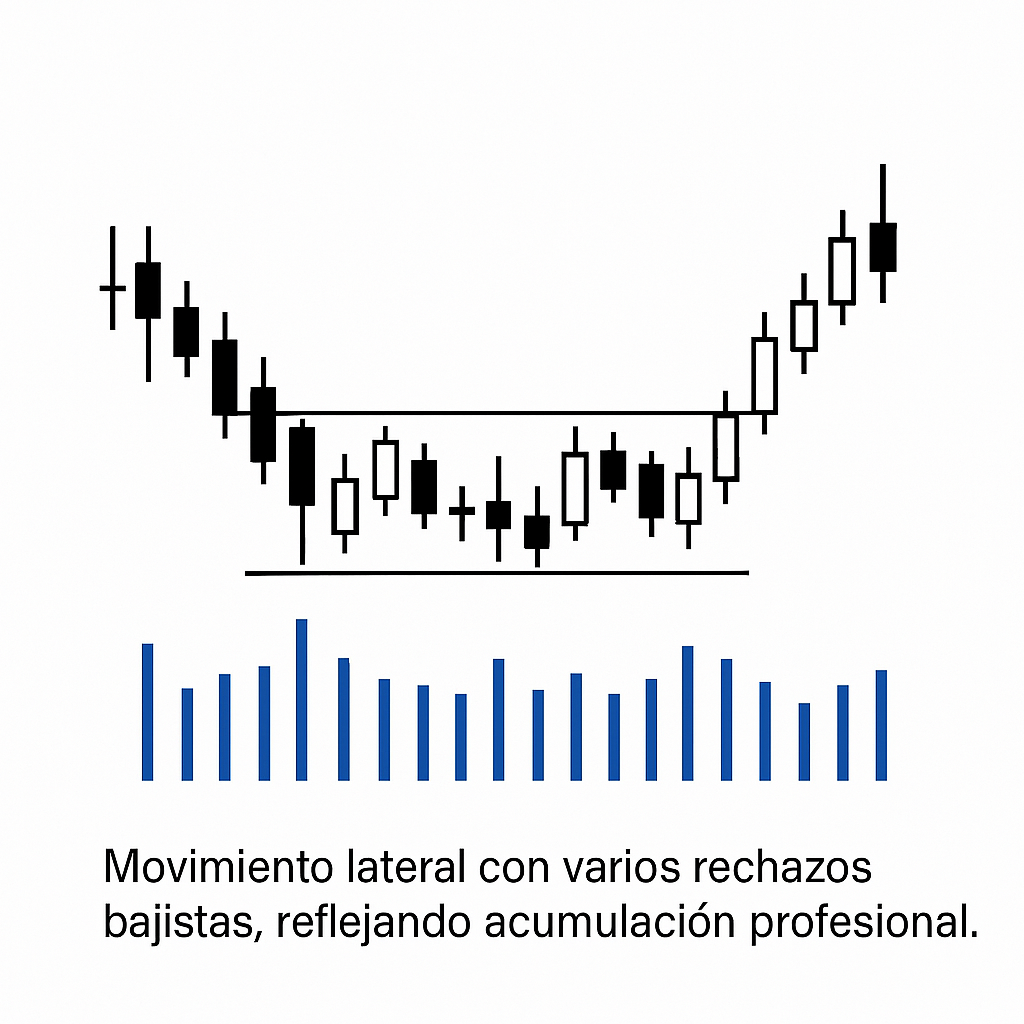
\includegraphics[width=11cm]{images/Acumulacion.png}
    \caption{Acumulaci\'on}
    \label{fig:Acumulacion}
\end{figure}

En la figura \ref{fig:Acumulacion} ...

\textbf{Distribuci\'on}: venta institucional en rangos estrechos en la parte alta del gr\'afico.
\subsubsection*{Distribuci\'on (Fase Profesional)}

\textbf{Descripci\'on textual:}

Proceso en el cual los operadores institucionales descargan posiciones (venden) en una zona de resistencia, generalmente tras una fase de tendencia alcista. Se caracteriza por:

\begin{itemize}
    \item Movimiento lateral con m\'aximos similares.
    \item Volumen alto sin progreso en el precio.
    \item Velas de rechazo bajista (\textit{pin bars}, \textit{engulfings}).
    \item Picos de volumen que coinciden con velas de cuerpo peque\~no o sombras superiores largas.
\end{itemize}

\begin{figure}[!htbp]
    \centering
    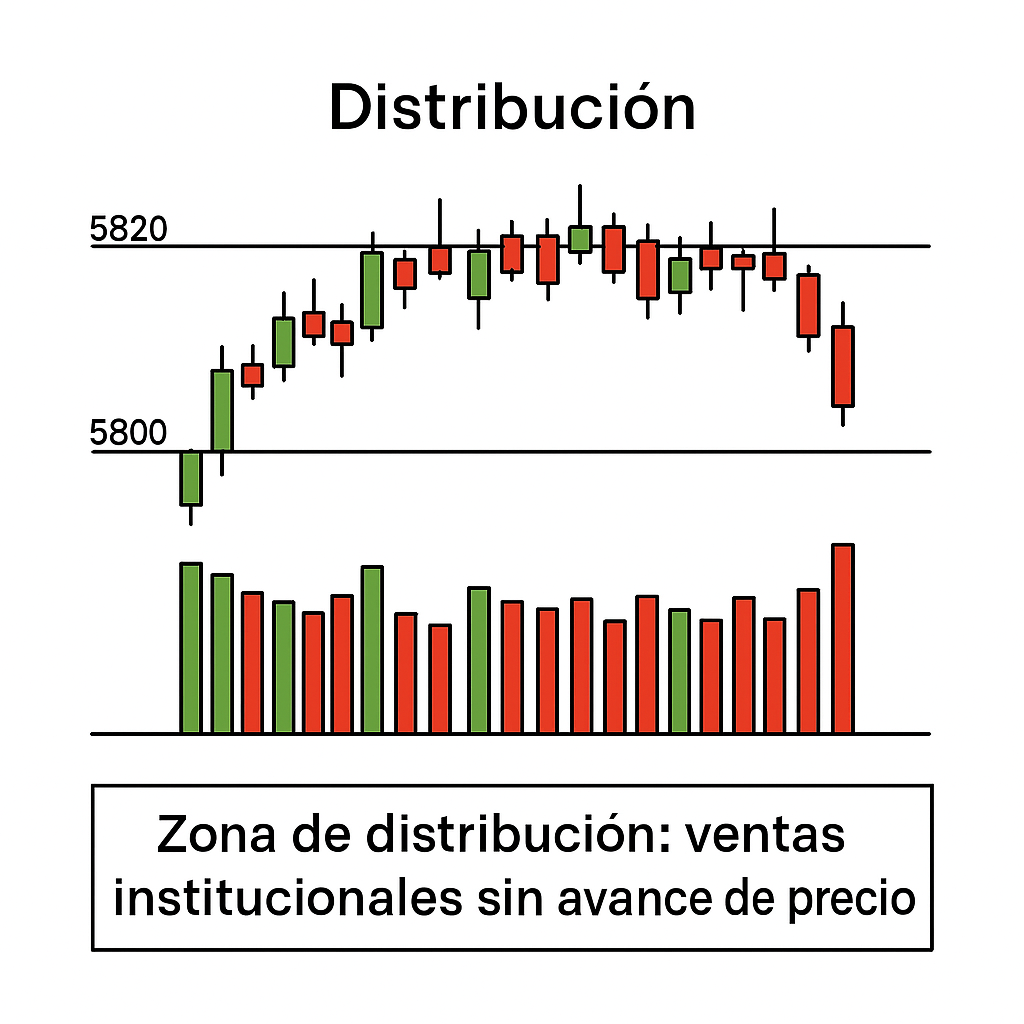
\includegraphics[width=11cm]{images/Distribucion.png}
    \caption{Distribuci\'on}
    \label{fig:Distribucion}
\end{figure}

En la figura \ref{fig:Distribucion} ...

Ambas fases implican una inversi\'on de tiempo y volumen significativos por parte del profesional, preparando movimientos posteriores mayores.

%\subsection{Caballo Ganador}

%Estructura fractal que combina impulsos y correcciones de distintos grados, todos en favor de un impulso principal. Sus claves:

%\begin{itemize}
%    \item Confirmaci\'on de cada subestructura por superaci\'on de niveles previos.
%    \item Objetivo: completar una segunda pata proporcional al impulso mayor.
%    \item Si una correcci\'on es superada, se confirma la continuaci\'on impulsiva.
%\end{itemize}

\section{An\'alisis de Velas}

El an\'alisis de velas, seg\'un Al Brooks, constituye una herramienta poderosa para entender la din\'amica subyacente del mercado, permitiendo interpretar la acci\'on del precio de manera profunda y eficaz. Brooks enfatiza la importancia del contexto, afirmando que ninguna vela debe analizarse de manera aislada; cada vela debe estudiarse considerando su posici\'on dentro de la tendencia global y el comportamiento precedente del precio.

\subsection{Velas de Intenci\'on}

Estas velas presentan un cuerpo amplio y cierran cerca de sus extremos superiores (si son alcistas) o inferiores (si son bajistas). Brooks considera que una vela de gran cuerpo refleja un sentimiento fuerte del mercado, con una clara dominancia por parte de compradores o vendedores. El volumen asociado a estas velas suele ser alto, indicando una fuerte participaci\'on institucional. Sin embargo, si una vela de intenci\'on aparece sin continuidad y con volumen decreciente, puede estar indicando una trampa o enga\~no de mercado.

\begin{figure}[!htbp]
    \centering
    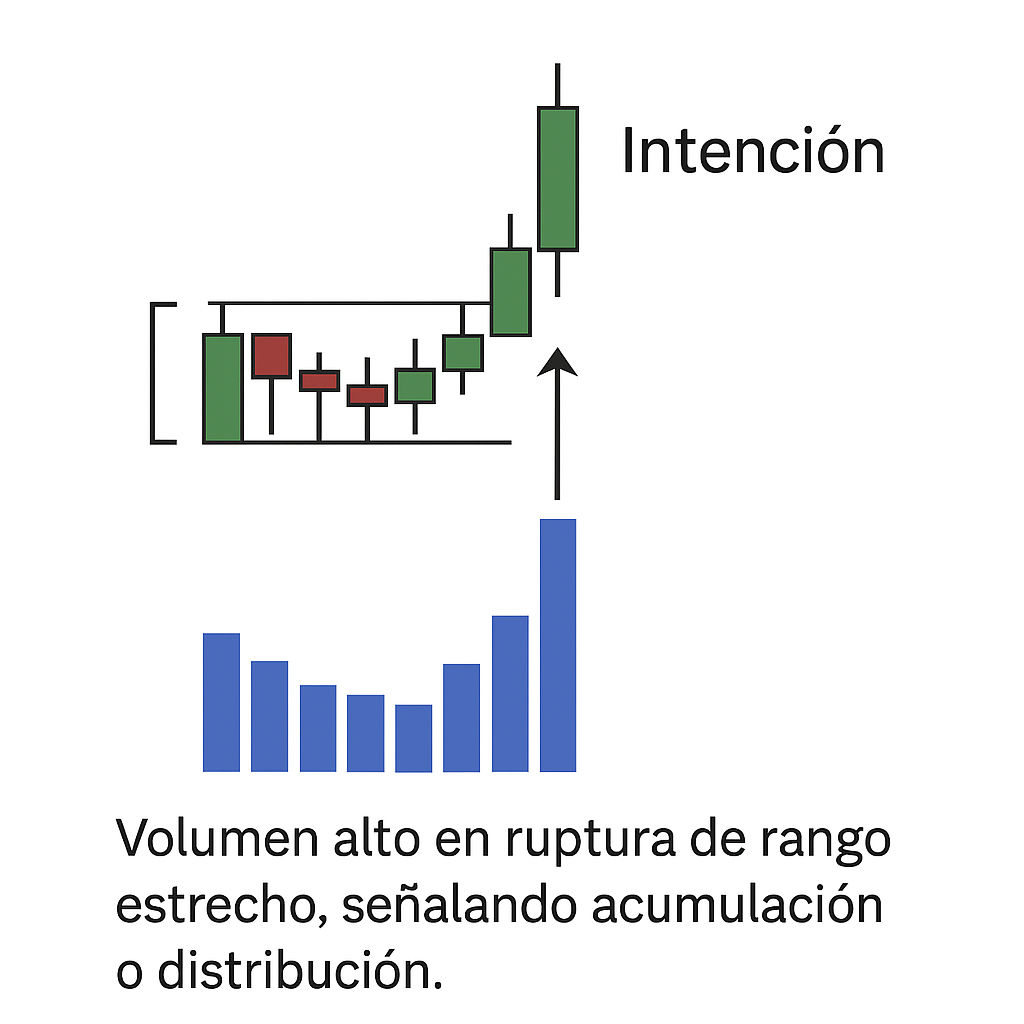
\includegraphics[width=11cm]{images/Intencion.png}
    \caption{Intenci\'on}
    \label{fig:Intencion2}
\end{figure}

En la figura \ref{fig:Intencion2} ...

\subsection{Velas Envolventes (Outside Bars)}

Una vela envolvente tiene un rango que excede tanto el m\'aximo como el m\'inimo de la vela anterior. Brooks indica que estas velas son complejas y deben analizarse con precauci\'on, pues pueden representar desde una pausa moment\'anea hasta un cambio de tendencia definitivo. Su relevancia aumenta considerablemente si aparecen tras movimientos prolongados, especialmente cuando capturan a operadores que entraron en velas anteriores, generando movimientos reactivos bruscos.

\begin{figure}[!htbp]
    \centering
    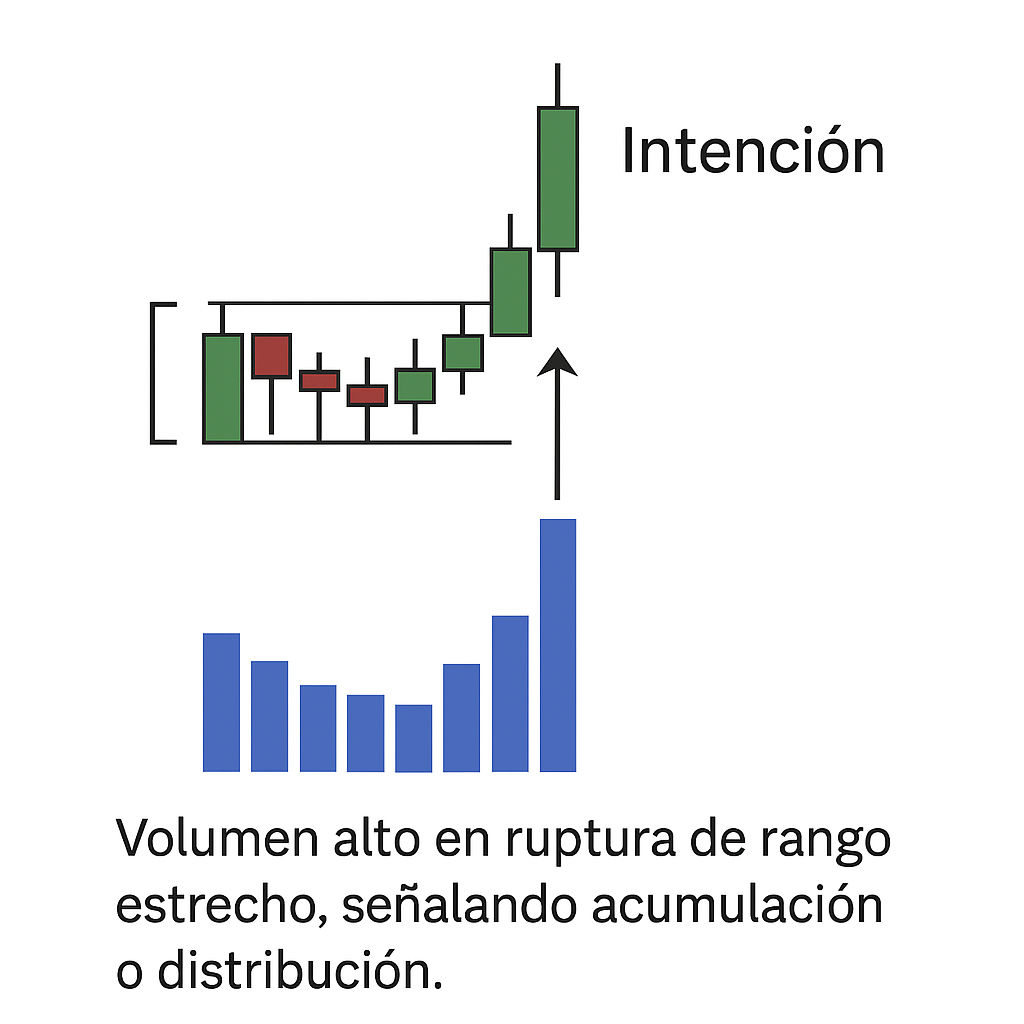
\includegraphics[width=11cm]{images/Intencion.png}
    \caption{Intenci\'on}
    \label{fig:Intencion3}
\end{figure}

En la figura \ref{fig:Intencion3} ...

\subsection{Velas de Rango Estrecho}

Estas velas, tambi\'en denominadas peonzas, muestran un cuerpo peque\~no y generalmente presentan mechas largas. Para Brooks, reflejan indecisi\'on o pausa, sugiriendo un agotamiento temporal de la fuerza impulsora predominante en el mercado. Cuando aparecen con volumen alto, son especialmente relevantes pues pueden indicar una absorci\'on significativa de \textit{oferta} o \textit{demanda}, alertando sobre posibles puntos de reversi\'on.

\subsection{Velas de Volumen Excesivo}

Caracterizadas por un cuerpo amplio acompa\~nado de un volumen extraordinariamente alto, estas velas a menudo esconden fuerza contraria. En una tendencia alcista, por ejemplo, una vela de este tipo podr\'ia implicar una distribuci\'on oculta por parte de operadores profesionales. Brooks recomienda analizar con cuidado estas velas dentro del contexto, especialmente en niveles extremos del gr\'afico.

\subsection{Velas Doji y Velas Inside}

Brooks se\~nala que las velas Doji, con apertura y cierre casi id\'enticos, representan una fuerte indecisi\'on del mercado. Cuando aparecen con volumen significativo, son potenciales precursoras de giros importantes. Las velas inside, contenidas completamente dentro del rango de la vela anterior, indican consolidaci\'on o equilibrio temporal. Pueden anticipar movimientos explosivos cuando son rotas con volumen elevado.

\subsection{Importancia del Contexto}

Al Brooks insiste en que el contexto define la validez de cualquier vela o patr\'on de velas. Una misma vela puede tener interpretaciones distintas seg\'un su ubicaci\'on dentro del ciclo del mercado. Por ejemplo, una vela envolvente en un mercado lateralizado tiene implicaciones diferentes a si ocurre tras una larga tendencia alcista o bajista.

\subsection{Integraci\'on con An\'alisis de Volumen}

Finalmente, es esencial validar la acci\'on del precio con volumen. Una vela alcista amplia debe estar respaldada por volumen alto para confirmar la intenci\'on profesional. Si el volumen es bajo, la vela podr\'ia ser una se\~nal falsa o manipulativa. Esta integraci\'on del an\'alisis de velas con el volumen es clave para la metodolog\'ia propuesta por Brooks, proporcionando un marco completo y robusto para la toma de decisiones operativas.

En resumen, el an\'alisis de velas seg\'un Al Brooks ofrece una visi\'on detallada y pragm\'atica para interpretar la din\'amica del mercado, enfatizando la importancia del contexto, el volumen y la acci\'on colectiva de las velas para anticipar movimientos futuros del precio.

\section{An\'alisis de Velas: Integrando los enfoques de Al Brooks y Miguel \'Angel Ram\'irez}

El an\'alisis de velas constituye una herramienta esencial para interpretar la acci\'on del precio. Tanto Miguel \'Angel Ram\'irez como Al Brooks enfatizan la importancia de estudiar la formaci\'on, estructura, volumen y contexto de las velas para detectar la intenci\'on profesional oculta detr\'as del movimiento del mercado.

Para ambos autores, las velas no deben interpretarse de forma aislada; es imprescindible considerar su contexto inmediato, la continuidad posterior al cierre y la relaci\'on con el volumen que las acompa\~na.

\subsection{La importancia del Contexto}

Al Brooks afirma que el significado de cada vela depende crucialmente de su ubicaci\'on en la estructura del mercado (tendencia, rango o transici\'on). Miguel \'Angel Ram\'irez, por su parte, coincide y enfatiza especialmente las \textbf{zonas relevantes} donde las velas adquieren mayor significaci\'on:

\begin{itemize}
    \item \textbf{Soportes y resistencias clave:} una vela alcista de intenci\'on con volumen alto en soporte revela acumulaci\'on profesional; en resistencia, una vela bajista de intenci\'on con alto volumen denota distribuci\'on.
    \item \textbf{Directrices mayores y menores:} velas que reaccionan claramente en estas l\'ineas de tendencia sugieren validaci\'on o ruptura profesional.
    \item \textbf{Patrones complejos (HCH, rangos laterales):} la ruptura o rechazo mediante velas de intenci\'on valida la presencia activa del profesional.
\end{itemize}

\subsection{Tipos de Velas y su interpretaci\'on operativa}

Al integrar ambos enfoques, se reconocen varios tipos espec\'ificos de velas y su significado desde la acci\'on profesional:

\subsubsection{Velas de Intenci\'on (Trend Bar - Brooks / Velas con Volumen Alto - Ram\'irez)}

Son velas con un cuerpo amplio, cierre en el extremo alto o bajo y con un volumen significativo. Ambas perspectivas coinciden en su interpretaci\'on:

\begin{itemize}
    \sloppy
    \item Indican clara dominancia de una de las fuerzas del mercado (compradores o vendedores).
    \item Son caracter\'isticas en rupturas genuinas de zonas relevantes (soportes, resistencias, directrices, rango).
    \item La ausencia inmediata de continuidad posterior puede indicar una trampa profesional (enga\~no).
\end{itemize}

Ejemplo: una vela grande alcista, que cierra cerca de m\'aximos y con alto volumen rompiendo un nivel relevante de resistencia, indica fuerte acumulaci\'on e intenci\'on profesional compradora. Sin embargo, si la siguiente vela revierte con volumen alto, puede indicar una trampa.

\subsubsection{Velas de Rango Estrecho o Peonzas}

Estas velas tienen cuerpos peque\~nos y volumen elevado. Seg\'un Ram\'irez, representan absorci\'on profesional; seg\'un Brooks, reflejan equilibrio temporal e indecisi\'on. Su interpretaci\'on conjunta es clara:

\begin{itemize}
    \item Indican pausa o potencial cambio de intenci\'on del mercado.
    \item La presencia de alto volumen confirma actividad profesional encubierta (acumulaci\'on o distribuci\'on oculta).
    \item Deben analizarse cuidadosamente en zonas relevantes, pues suelen anticipar movimientos explosivos posteriores.
\end{itemize}

Ejemplo: Una peonza con alto volumen en la parte alta de un rango indica posible distribuci\'on encubierta antes de una ca\'ida importante del mercado.

\subsubsection{Velas de Volumen Excesivo (Exhaustion Bar - Brooks)}

Seg\'un ambos autores, estas velas muestran cuerpos muy amplios con volumen exageradamente alto, indicando sobreesfuerzo y posible cl\'imax del movimiento vigente:

\begin{itemize}
    \item Brooks las describe como velas clim\'aticas, marcando agotamiento.
    \item Ram\'irez advierte que en niveles extremos pueden ocultar intenciones contrarias: los profesionales rara vez compran agresivamente en techos ni venden agresivamente en fondos.
    \item La falta de continuidad posterior confirma agotamiento y potencial giro del mercado.
\end{itemize}

Ejemplo: una vela clim\'atica alcista con volumen extremadamente alto tras una fuerte tendencia alcista puede se\~nalar distribuci\'on profesional previa a un giro bajista.

\subsection*{Puntos en Com\'un}

\begin{enumerate}
    \item \textbf{Aparici\'on tras movimientos prolongados:}
    \begin{itemize}
        \item Ambas velas suelen adquirir mayor relevancia cuando se presentan \textbf{al final de una tendencia fuerte}.
        \item En ese contexto, act\'uan como se\~nales potenciales de \textbf{cambio de fase}: transici\'on de tendencia a rango o reversi\'on.
    \end{itemize}

    \item \textbf{Lectura de agotamiento o trampa:}
    \begin{itemize}
        \item La \textbf{vela envolvente}, si no tiene continuaci\'on, puede reflejar \textbf{una trampa} o \textbf{absorci\'on profesional}.
        \item La \textbf{vela de volumen excesivo} tambi\'en sugiere un \textbf{cl\'imax de agotamiento}, donde los profesionales \textbf{capturan liquidez} de \textit{traders} minoristas.
    \end{itemize}

    \item \textbf{Advertencia de reversi\'on inminente:}
    \begin{itemize}
        \item Ambas velas pueden se\~nalar que el \textbf{movimiento vigente est\'a maduro o agotado}, y que existe un riesgo elevado de giro.
        \item En especial si van seguidas de falta de continuaci\'on o de una vela contraria fuerte.
    \end{itemize}

    \item \textbf{Necesidad de validaci\'on contextual:}
    \begin{itemize}
        \item Ni la vela envolvente ni la de volumen excesivo deben operar por s\'i solas: su interpretaci\'on requiere el \textbf{an\'alisis del contexto estructural y del volumen}.
        \item Ambas pueden fallar si se interpretan fuera de zonas relevantes (resistencias, soportes, extremos de canales).
    \end{itemize}

    \item \textbf{Captura de operadores mal posicionados:}
    \begin{itemize}
        \item Las dos velas suelen estar asociadas a \textbf{movimientos que atrapan} a quienes entraron tarde, lo que genera \textbf{reacciones violentas} en sentido contrario.
    \end{itemize}
\end{enumerate}

\subsection*{Conclusi\'on}

Ambos tipos de velas deben ser interpretados como \textbf{manifestaciones del comportamiento profesional} al final de un tramo de mercado. Aunque se enfocan en aspectos distintos (estructura vs.\ volumen), \textbf{convergen en su utilidad como se\~nales de agotamiento, manipulaci\'on o transici\'on}, especialmente en zonas t\'ecnicas clave.


\subsubsection{Velas de Rechazo (Reversal Bar - Brooks)}

Estas velas presentan largas sombras superiores o inferiores y cuerpo peque\~no a medio. Para Ram\'irez, estas velas aparecen en «testeos» para comprobar la presencia contraria. Para Brooks, significan un claro rechazo a un nivel espec\'ifico:

\begin{itemize}
    \item Una sombra inferior larga en un soporte relevante indica rechazo a precios m\'as bajos y posible comienzo de acumulaci\'on profesional.
    \item Una sombra superior larga en resistencia relevante denota rechazo de precios altos y posible inicio de distribuci\'on profesional.
    \item La confirmaci\'on mediante la siguiente vela es fundamental para validar o descartar la reversi\'on del movimiento.
\end{itemize}

Ejemplo: una vela bajista con sombra inferior muy larga sobre un soporte importante, seguida de una vela alcista de intenci\'on con volumen, indica acumulaci\'on validada y giro alcista.

\subsection{Integraci\'on operativa: Precio y Volumen}

La integraci\'on del volumen en el an\'alisis de velas potencia enormemente la capacidad predictiva del trader:

\begin{itemize}
    \item Las velas de intenci\'on deben ir acompa\~nadas siempre de volumen alto para ser consideradas v\'alidas; ausencia de volumen implica falsa ruptura o trampa profesional.
    \item Velas de rango estrecho con volumen alto indican absorci\'on profesional, anticipando movimientos significativos.
    \item Las velas clim\'aticas (excesivas) siempre tienen volumen exagerado, confirmando agotamiento.
\end{itemize}

Ambos enfoques coinciden plenamente en que el volumen aporta confirmaci\'on y seguridad operativa.

\subsection{Confirmaci\'on y Continuidad}

Para Brooks y Ram\'irez es clave la continuidad posterior a cualquier vela relevante:

\begin{itemize}
    \item Una vela fuerte (intenci\'on) requiere continuidad inmediata; su ausencia sugiere una trampa.
    \item Las velas de rechazo deben ser seguidas de velas confirmatorias en direcci\'on contraria al rechazo.
    \item Velas clim\'aticas deben mostrar rechazo inmediato al movimiento previo para confirmar el agotamiento.
\end{itemize}

\subsection{Conclusi\'on Integradora}

La combinaci\'on de las perspectivas de Al Brooks y Miguel \'Angel Ram\'irez en el an\'alisis de velas proporciona un enfoque potente y detallado para interpretar adecuadamente el mercado. Al observar la interacci\'on entre contexto, fuerza relativa (forma y tama\~no), continuidad y volumen, el trader obtiene una lectura clara de las verdaderas intenciones profesionales, logrando as\'i anticiparse a movimientos importantes y evitando trampas comunes en los mercados financieros.

Este an\'alisis profundo permite al operador actuar del lado correcto del mercado, alineado con las fuerzas institucionales y aumentando significativamente sus probabilidades de \'exito.

\section{Zonas Relevantes: Profundizaci\'on Operativa}

Las \textbf{zonas relevantes} constituyen niveles clave donde la interacci\'on del precio y el volumen revela con claridad la actividad profesional y permite tomar decisiones operativas precisas. Miguel \'Angel Ram\'irez y Al Brooks enfatizan que el correcto reconocimiento y an\'alisis de estas zonas representa uno de los pilares fundamentales del trading profesional basado en la acci\'on del precio.

Estas zonas no son simples l\'ineas est\'aticas, sino \textbf{\'areas din\'amicas} donde la lucha entre oferta y demanda genera patrones espec\'ificos y reveladores.

\subsection{Soportes y Resistencias Clave}

Seg\'un ambos autores, soportes y resistencias relevantes no son niveles fijos, sino rangos donde los profesionales han demostrado inter\'es significativo, ya sea mediante acumulaci\'on (compras institucionales) o distribuci\'on (ventas institucionales):

\begin{itemize}
    \item \textbf{Soporte relevante:} Un nivel o rango inferior del gr\'afico en el que, reiteradamente, el precio ha detenido su descenso. La presencia profesional se revela mediante velas de rechazo con volumen alto o testeos con secado de volumen.
    
    \item \textbf{Resistencia relevante:} Nivel o rango superior donde el precio repetidamente se ha detenido en su ascenso. Suele revelarse mediante velas de rechazo bajista, velas de rango estrecho con volumen alto (absorci\'on) o secado posterior a testeos alcistas fallidos.
    
    \item \textbf{Validaci\'on del nivel relevante:} Seg\'un Ram\'irez, un soporte recuperado con volumen e intenci\'on es la se\~nal m\'as clara de fortaleza. De manera an\'aloga, una resistencia dilatada con volumen sugiere clara debilidad y posible reversi\'on bajista.
\end{itemize}

\vspace{1em}
\noindent

\begin{figure}[!htbp]
    \centering
    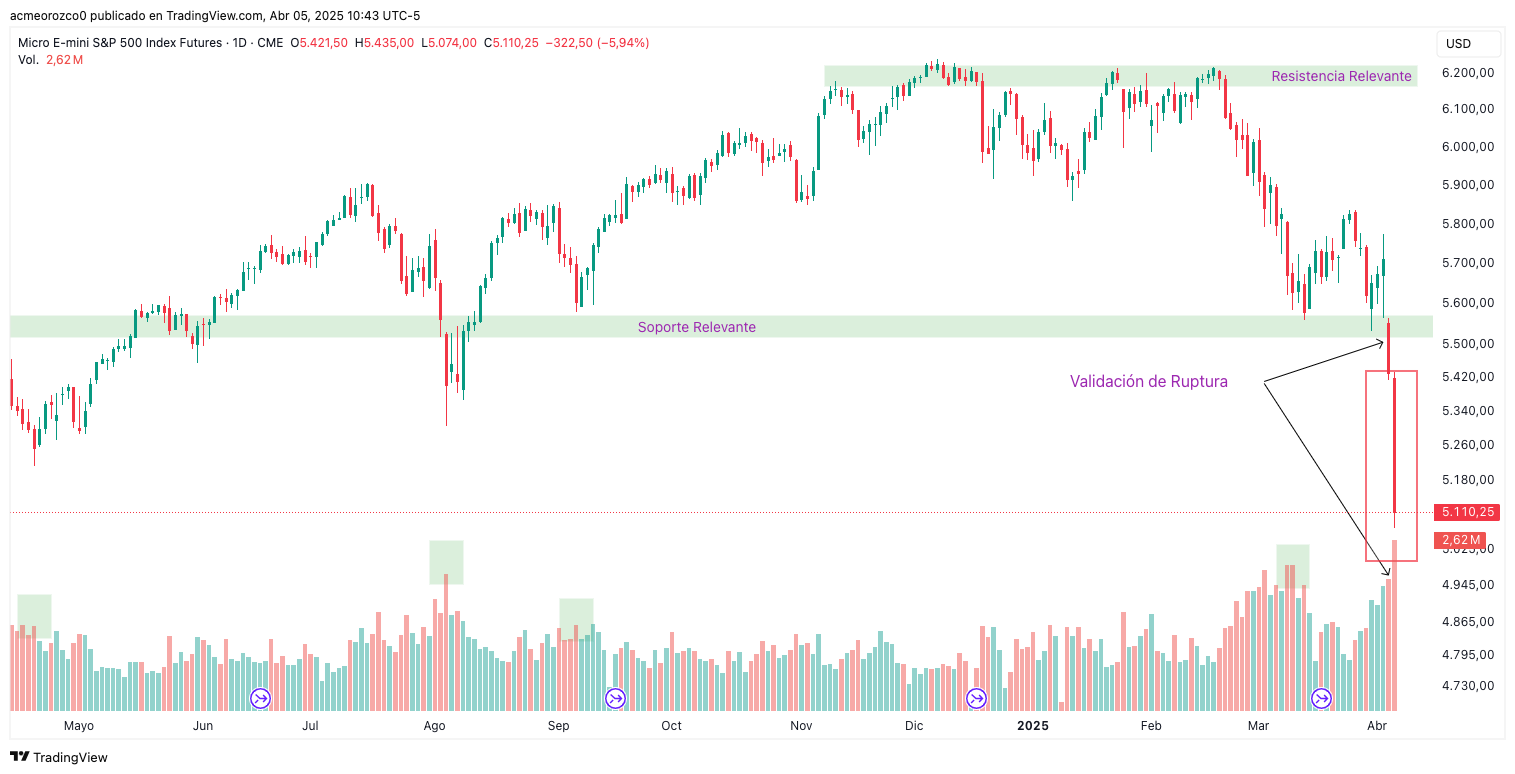
\includegraphics[width=11cm]{images/soportes_resistencias_validacion.png}
    \caption{Soporte, Resistencia y validaci\'on de Ruptura de Zona Clave}
    \label{fig:soportes_resistencias_validacion}
\end{figure}
\vspace{0.5em}
\noindent

\subsection{Interpretaci\'on del Gr\'afico, figura \ref{fig:soportes_resistencias_validacion}: Soportes, Resistencias y Validaci\'on}

La imagen anotada representa visualmente el concepto de \textbf{Soportes y Resistencias Clave}, aplicado al contrato diario del \textbf{MES-0625 (Micro E-mini S\&P 500 Futures)}. A continuaci\'on se detalla la lectura t\'ecnica de cada elemento:

\subsubsection*{Soporte relevante}

\textbf{Ubicaci\'on:} Zona horizontal entre 5.570 y 5.500 puntos, marcada con un recuadro verde con la anotaci\'on ``Soporte Relevante''.

\begin{itemize}
    \item Esta \'area muestra varios \textbf{rebotes del precio} tras ca\'idas, indicando la presencia de demanda institucional.
    \item Es una regi\'on donde se ha evidenciado \textbf{acumulaci\'on profesional}, seg\'un Ram\'irez, observable por:
    \begin{itemize}
        \item Velas con sombras inferiores largas (rechazo del precio a seguir cayendo).
        \item Incremento del volumen en los rebotes.
    \end{itemize}
    \item Act\'ua como \textbf{zona de defensa} del mercado: cada contacto del precio con esta zona activa la intervenci\'on de compradores profesionales.
\end{itemize}

\subsubsection*{Resistencia relevante}

\textbf{Ubicaci\'on:} Rango entre 6.150 y 6.220 puntos, señalado con un recuadro verde.

\begin{itemize}
    \item Este nivel funciona como techo t\'ecnico, deteniendo el avance del precio en m\'ultiples ocasiones.
    \item Se observa \textbf{distribuci\'on profesional} por medio de:
    \begin{itemize}
        \item Velas de rango estrecho con volumen alto (absorci\'on).
        \item Rechazos bajistas tras testeos fallidos.
    \end{itemize}
    \item La incapacidad del precio de mantenerse por encima de esta zona refuerza su condici\'on de resistencia clave.
\end{itemize}

\subsubsection*{Validaci\'on bajista del soporte}

\textbf{Ubicaci\'on:} Vela del 4 de abril de 2025, marcada con un recuadro rojo.

\begin{itemize}
    \item Se trata de una \textbf{vela bajista de cuerpo amplio}, con un volumen excepcional de \textbf{2{,}62 millones de contratos}.
    \item Representa una \textbf{ruptura con intenci\'on} del soporte, seg\'un el criterio de Miguel \'Angel Ram\'irez.
    \item El movimiento vertical y la falta de rechazo sugieren \textbf{dominancia de la oferta institucional}.
    \item Esto valida la \textbf{debilidad del nivel}, abriendo paso a una fase tipo \textit{markdown}.
\end{itemize}

\subsubsection*{Conclusi\'on operativa}

Este gr\'afico constituye un ejemplo pr\'actico del modelo de lectura institucional:

\begin{itemize}
    \item Identificaci\'on de zonas de inter\'es profesional (soporte y resistencia).
    \item Observaci\'on del comportamiento del precio ante dichos niveles.
    \item Confirmaci\'on mediante \textbf{intenci\'on y volumen} para validar rupturas o rechazos.
\end{itemize}

Este tipo de lectura permite al operador alinear sus decisiones con el flujo profesional del mercado.

\subsection{L\'ineas de Tendencia (Directrices)}

Al Brooks resalta la importancia operativa de las l\'ineas de tendencia como zonas din\'amicas, mientras Ram\'irez se enfoca en identificar la intenci\'on profesional en estas directrices:

\begin{itemize}
    \item Una l\'inea de tendencia efectiva conecta m\'ultiples puntos donde los profesionales actuaron previamente (acumulaci\'on o distribuci\'on).
    
    \item Para que una ruptura de directriz sea fiable, debe hacerse con \textbf{intenci\'on}: vela de amplio rango, cierre decidido m\'as all\'a de la directriz y aumento significativo del volumen. De lo contrario, se trata de un testeo o dilataci\'on (trampa profesional).
    
    \item Una l\'inea de tendencia rota con intenci\'on revela cambios potencialmente profundos en la estructura del mercado, indicando transici\'on desde una fase impulsiva a correctiva o viceversa.
\end{itemize}

\subsubsection{L\'ineas de Tendencia (Directrices) en el MES-0625}

En la siguiente imagen, \ref{fig:lineas_tendencia_directrices}, se ilustran dos \textbf{directrices clave} que reflejan la acci\'on institucional sobre el contrato \textbf{MES-0625} en el marco diario, junto con una \textbf{ruptura con intenci\'on} que valida un cambio estructural del mercado:


\vspace{1em}
\noindent

\begin{figure}[!htbp]
    \centering
    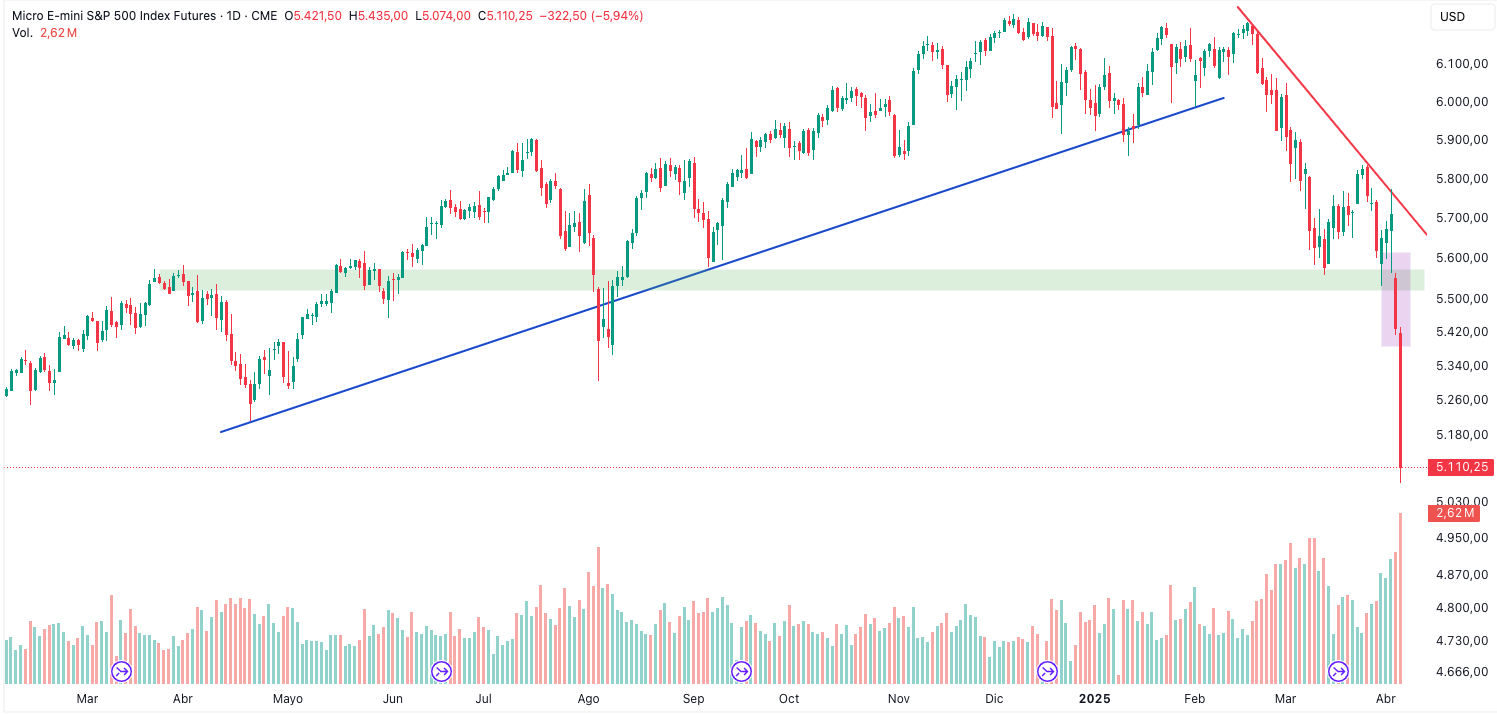
\includegraphics[width=11cm]{images/lineas_tendencia_directrices.png}
    \caption{L\'ineas de Tendencia (Directrices) en el MES-0625 y Ruptura de Zona Clave}
    \label{fig:lineas_tendencia_directrices}
\end{figure}
\vspace{0.5em}
\noindent

\begin{itemize}
    \item \textbf{Directriz alcista (azul):} conecta los m\'inimos ascendentes desde octubre de 2023 hasta abril de 2024. Esta l\'inea representa una fase de \textbf{acumulaci\'on profesional}, donde la demanda institucional sosten\'ia el mercado. Su pendiente refleja una estructura de m\'inimos crecientes, t\'ipica de una fase impulsiva alcista.
    
    \item \textbf{Directriz bajista (roja):} une los m\'aximos descendentes desde inicios de 2025 hasta marzo–abril del mismo a\~no. Esta estructura indica una fase de \textbf{distribuci\'on}, donde la oferta comienza a dominar lentamente el mercado, frenando los impulsos alcistas y anticipando un giro.
    
    \item \textbf{Ruptura con intenci\'on (recuadro morado):} el 4 de abril de 2025 se observa una \textbf{vela de amplio rango bajista} que rompe de forma decidida el soporte relevante. Esta vela est\'a acompa\~nada por un volumen hist\'oricamente alto (2{,}62 millones de contratos), cumpliendo con los criterios de Ram\'irez para validar una ruptura con intenci\'on:
    \begin{itemize}
        \item Cuerpo amplio y direccional.
        \item Cierre por debajo de la directriz.
        \item Volumen extraordinario.
    \end{itemize}
    Esta ruptura sugiere el paso desde una fase de \textbf{distribuci\'on} a una \textbf{fase impulsiva bajista} o \textit{markdown}.
\end{itemize}

\vspace{1em}
\noindent
Este tipo de lectura sobre las directrices permite anticipar cambios de fase del mercado y validar la presencia profesional en zonas clave, fortaleciendo la estrategia operativa basada en acci\'on del precio y volumen.


\subsection{Patrones Complejos y Zonas Claviculares}

Miguel \'Angel Ram\'irez enfatiza la importancia de los \textbf{patrones complejos}, como el Hombro-Cabeza-Hombro (HCH), dobles techos y estructuras compuestas, como manifestaciones t\'ipicas de \textbf{distribuci\'on o acumulaci\'on profesional} en zonas t\'ecnicas clave. En este marco, el concepto de \textbf{zona clavicular} adquiere un rol operativo fundamental.

\begin{itemize}
    \item La \textbf{clavicular} es una l\'inea que conecta los \textbf{m\'inimos en patrones alcistas} o los \textbf{m\'aximos en patrones bajistas}, actuando como \textbf{nivel din\'amico de equilibrio} entre oferta y demanda. En t\'erminos funcionales, representa la frontera que, una vez rota con convicci\'on, habilita desplazamientos impulsivos.

    \item La clavicular conecta puntos cr\'iticos (m\'inimos en patrones alcistas o m\'aximos en bajistas), formando niveles din\'amicos clave.  
    \item Una ruptura clara de la clavicular con volumen alto valida el patr\'on y anticipa movimientos de gran amplitud. Ausencia de volumen sugiere falsa ruptura o testeo fallido.    
    \item Ram\'irez recomienda trazar la clavicular no solo en el grado mayor, sino tambi\'en en el grado menor m\'as reciente, aumentando la precisi\'on operativa.
    \item Una \textbf{ruptura con volumen alto e intenci\'on clara} valida el patr\'on y suele anticipar movimientos amplios y definidos. Este elemento es esencial para distinguir entre una \textbf{ruptura genuina} y una \textbf{falsa ruptura} o \textit{trampa institucional}, cuando la acci\'on carece de volumen o continuidad.
    \item Ram\'irez propone un an\'alisis multigrado: no basta con trazar la clavicular en el patr\'on visible de mayor jerarqu\'ia, sino que tambi\'en debe identificarse la \textbf{clavicular del patr\'on interno m\'as reciente}. Esta pr\'actica permite:
    \begin{itemize}
        \item Mejorar la \textbf{precisi\'on en las entradas}.
        \item Detectar anticipadamente \textbf{fallos estructurales} o \textbf{confirmaciones operativas}.
    \end{itemize}
    \item Las zonas claviculares tambi\'en permiten evaluar el \textbf{rol de testeo}, ya que un retroceso hacia la clavicular rota puede validar la ruptura si se acompa\~na de secado de volumen o rechazo (intenci\'on inversa).
    \item Las zonas claviculares tambi\'en son v\'alidas como \textbf{zonas de testeo posterior a la ruptura}. Un retroceso controlado hacia la clavicular rota, con \textbf{secado de volumen o rechazo}, puede confirmar la intenci\'on profesional y habilitar una entrada en favor del movimiento validado.
\end{itemize}

\noindent
Este abordaje profundo de las zonas claviculares se integra al enfoque institucional de Ram\'irez, quien no las utiliza como patrones autom\'aticos, sino como \textbf{zonas vivas}, en las que la lectura del volumen, el contexto previo y la continuidad posterior determinan su validez como punto de transici\'on estructural.

\vspace{1em}
\noindent
\begin{figure}[!htbp]
    \centering
    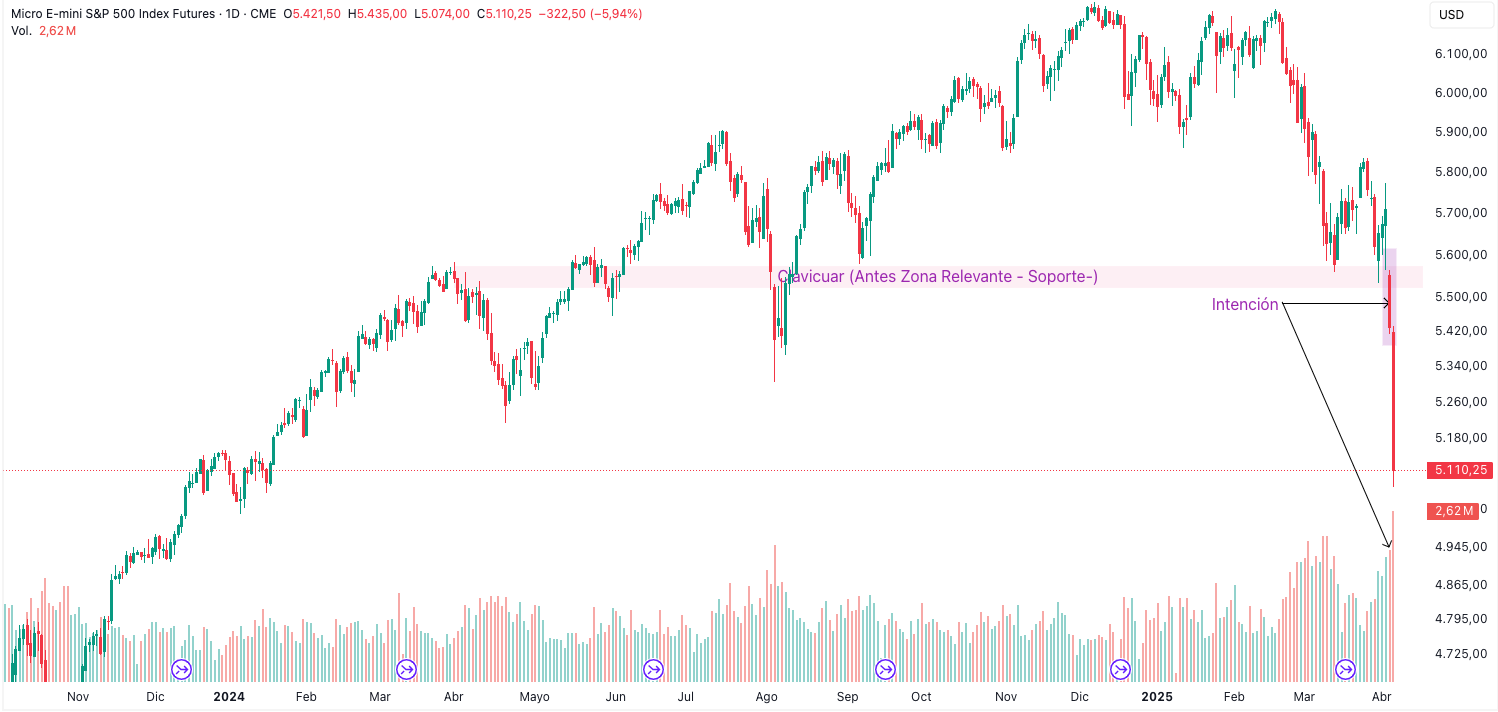
\includegraphics[width=11cm]{images/patrones_claviculares_test_ruptura.png}
    \caption{Estructura de clavicular, testeo previo y ruptura con volumen en el MES-0625}
    \label{fig:patrones_claviculares_test_ruptura}
\end{figure}
\vspace{0.5em}
\noindent


En la figura \ref{fig:patrones_claviculares_test_ruptura} se observa un ejemplo operativo del concepto de \textbf{zonas claviculares} aplicado al contrato \textbf{MES-0625} en marco diario. La estructura muestra un patr\'on complejo tipo Hombro-Cabeza-Hombro, seguido de una ruptura validada por volumen. Se identifican los siguientes elementos:

\begin{itemize}
    \item \textbf{Clavicular:} traza la l\'inea que conecta los m\'inimos clave de la estructura completa, actuando como frontera principal entre la fase de distribuci\'on y el potencial movimiento impulsivo bajista.

    \item \textbf{Testeo:} antes de la ruptura definitiva, el precio realiza un retroceso que pone a prueba la zona clavicular, valid\'andola mediante rechazo con bajo volumen.

    \item \textbf{Ruptura con Volumen:} la vela del 4 de abril de 2025 rompe la clavicular (antes Zona Relevante ---Soporte--- ) con cuerpo amplio y volumen hist\'orico (2{,}62 millones de contratos), confirmando la intenci\'on institucional y validando el patr\'on bajista.
\end{itemize}

\noindent
Este tipo de lectura secuencial permite detectar y operar transiciones estructurales reales, evitando falsas rupturas y posicionando al operador en sincron\'ia con la acci\'on profesional del mercado.


\subsection{Zonas de Acumulaci\'on y Distribuci\'on}

Estas zonas son centrales en el an\'alisis de Ram\'irez y respaldadas indirectamente por Brooks mediante su interpretaci\'on contextual:

\begin{itemize}
    \item \textbf{Zonas de Acumulaci\'on:} Identificadas en la parte baja del gr\'afico, caracterizadas por movimientos laterales con volumen alto en velas de rango estrecho (absorci\'on). La salida alcista posterior, con velas de intenci\'on y volumen relevante, confirma la acumulaci\'on previa. Ram\'irez describe estas zonas como estructuras laterales que se forman tras prolongadas ca\'idas, usualmente en la parte baja del gr\'afico. En ellas, el operador profesional \textbf{absorbe oferta} mediante velas de rango estrecho y volumen elevado. La salida posterior mediante velas de intenci\'on con volumen creciente valida dicha acumulaci\'on. Este enfoque coincide con la lectura contextual de Brooks, quien se enfoca en \textbf{rangos en la base con ruptura impulsiva y continuidad}.
    
    \item \textbf{Zonas de Distribuci\'on:} Encontradas en la parte alta del gr\'afico, con movimientos laterales similares pero con actividad vendedora oculta. Confirmadas cuando aparecen velas bajistas fuertes con alto volumen rompiendo soportes internos del rango lateral. Estas estructuras se configuran en los techos del mercado. Seg\'un Ram\'irez, el profesional \textbf{vende sin mover el precio}, generando una aparente lateralidad. La ruptura bajista posterior, con volumen alto y velas de amplio rango, confirma la distribuci\'on. Brooks, desde su an\'alisis de rango y reversi\'on en extremos, tambi\'en reconoce este comportamiento, aunque lo interpreta desde el \textbf{cambio de probabilidad en zonas de resistencia}.
    
    \item \textbf{Duraci\'on y volumen acumulado:} Ram\'irez enfatiza que \textbf{a mayor duraci\'on y volumen en la fase de acumulaci\'on o distribuci\'on}, mayor ser\'a la energ\'ia liberada una vez se valide la ruptura. Este principio est\'a vinculado con la \textbf{ley de causa y efecto}, y se proyecta directamente en la magnitud del desplazamiento posterior. Brooks, por su parte, indica que \textbf{cuanto m\'as testado un rango, m\'as fuerte suele ser su ruptura si hay confirmaci\'on de volumen e intenci\'on}. Cuanto mayor es el tiempo y volumen invertido en acumulaci\'on o distribuci\'on, m\'as potente ser\'a el movimiento resultante una vez que se rompa definitivamente dicha zona.
\end{itemize}

\noindent
Esta integraci\'on te\'orica refuerza la utilidad operativa de estas zonas como puntos estructurales clave, donde la lectura combinada de \textbf{volumen, acci\'on del precio y continuidad} permite identificar de manera anticipada la participaci\'on profesional y proyectar movimientos de alta probabilidad.


\vspace{1em}
\noindent
\begin{figure}[!htbp]
    \centering
    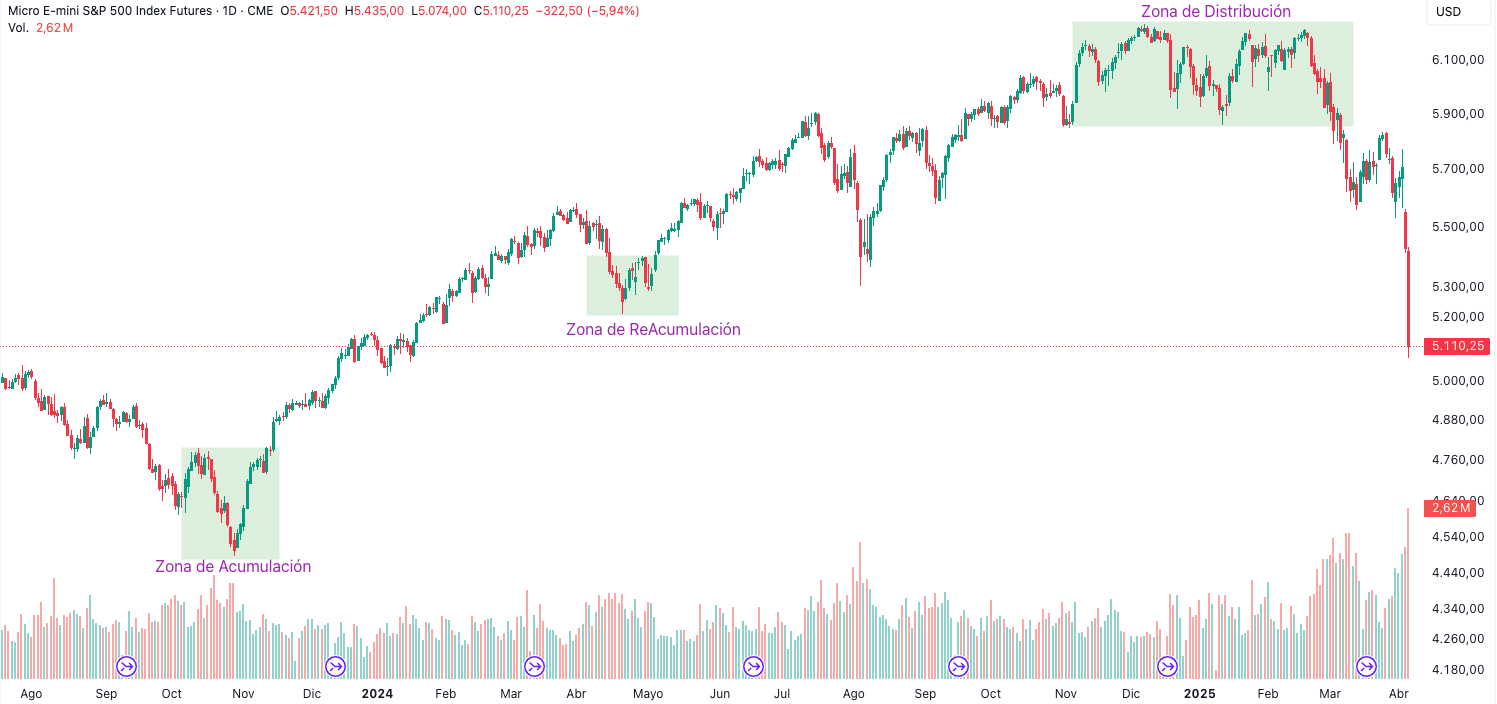
\includegraphics[width=11cm]{images/zonas_acumulacion_distribucion.png}
    \caption{Zonas de acumulaci\'on y distribuci\'on profesional en el MES-0625}
    \label{fig:zonas_acumulacion_distribucion}
\end{figure}
\vspace{0.5em}

\noindent
En la figura \ref{fig:zonas_acumulacion_distribucion} se ilustran dos zonas estructurales clave identificadas a partir del an\'alisis de \textbf{precio y volumen}, tal como lo propone \textbf{Miguel \'Angel Ram\'irez}, y que encuentran respaldo t\'acito en la lectura contextual de \textbf{Al Brooks}.

\begin{itemize}
    \item \textbf{Zona de Acumulaci\'on:} ubicada en la parte baja del gr\'afico, entre octubre de 2023 y noviembre de 2023. Se caracteriza por una fase lateral tras una ca\'ida prolongada, con velas de rango estrecho y volumen elevado, lo cual sugiere \textbf{absorci\'on profesional}. La salida alcista posterior, mediante velas de intenci\'on con volumen creciente, valida esta fase como acumulativa.

    \item \textbf{Zona de Distribuci\'on:} situada en el techo del mercado, entre noviembre de 2024 y febrero de 2025. Presenta un comportamiento lateral sin continuidad alcista, lo que indica \textbf{actividad vendedora encubierta}. La confirmaci\'on se da cuando el precio rompe los soportes internos del rango con una vela bajista de amplio rango y volumen extremo, iniciando una fase impulsiva descendente.

    \item \textbf{Principio de causa y efecto:} tal como sostiene Ram\'irez, \textbf{a mayor duraci\'on y volumen en estas zonas, mayor energ\'ia tendr\'a el movimiento posterior}. Este principio se observa en ambos casos, donde los desplazamientos posteriores fueron amplios y decididos.
\end{itemize}

\noindent
Estas zonas reflejan la participaci\'on activa del operador institucional y constituyen una herramienta de alta precisi\'on para anticipar transiciones estructurales en el mercado. Su correcta identificaci\'on permite actuar en sinton\'ia con la intenci\'on profesional y proyectar movimientos de alta probabilidad.



\subsection{Dilataciones y Falsas Rupturas}

Ambos autores coinciden en que las falsas rupturas (dilataciones) constituyen una herramienta estrat\'egica para los profesionales:

\begin{itemize}
    \item Las dilataciones se caracterizan por romper brevemente soportes o resistencias sin continuidad posterior, generando trampas que inducen al error a traders menos experimentados.
    
    \item Son reconocibles por el bajo volumen de ruptura, velas de rechazo inmediatas o por la falta de continuidad tras la vela inicial de ruptura.
    
    \item Detectar estas dilataciones tempranamente permite identificar los niveles verdaderos de acumulaci\'on o distribuci\'on profesional.
\end{itemize}


\subsection{Dilataciones y Falsas Rupturas}

Tanto Miguel \'Angel Ram\'irez como Al Brooks reconocen que las \textbf{dilataciones} o \textbf{falsas rupturas} son maniobras recurrentes del operador profesional para inducir a error al trader minorista y redistribuir la liquidez. Se trata de movimientos en apariencia decisivos que, al no presentar confirmaci\'on o continuidad posterior, revelan su naturaleza manipulativa.

\begin{itemize}
    \sloppy
    \item Las \textbf{dilataciones} ocurren cuando el precio rompe brevemente un soporte o resistencia relevante, para luego regresar r\'apidamente al rango anterior. Este comportamiento genera falsas se\~nales de ruptura que suelen \textbf{activar stops}, inducir entradas precipitadas y provocar reacciones emocionales en los operadores menos preparados.

    \item Ram\'irez describe estas maniobras como \textbf{trampas profesionales}, orientadas a \textbf{capturar liquidez} antes de realizar el movimiento verdadero. Estas rupturas se producen sin el respaldo de un volumen significativo ni de velas con intenci\'on clara, lo que las distingue de las rupturas aut\'enticas.

    \item Al Brooks, desde su perspectiva de acci\'on del precio pura, hace \'enfasis en que la ruptura de un nivel debe ser evaluada en funci\'on del \textbf{contexto previo} y la \textbf{reacci\'on inmediata posterior}. La falta de continuidad o la aparici\'on de una vela contraria fuerte suele ser indicio de una dilataci\'on.

    \item Los elementos t\'ecnicos que permiten identificar estas dilataciones incluyen:
    \begin{itemize}
        \item \textbf{Volumen bajo} en la ruptura o ruptura con volumen inusual pero sin continuidad.
        \item \textbf{Velas de rechazo inmediato}, con cuerpo estrecho y sombra larga en direcci\'on contraria.
        \item \textbf{Retorno r\'apido al rango} anterior o al canal previo.
    \end{itemize}

    \item Detectar estas maniobras permite al operador interpretar correctamente el \textbf{nivel real de inter\'es profesional} (acumulaci\'on o distribuci\'on), y aprovechar el enga\~no institucional como oportunidad operativa.
\end{itemize}

\noindent
En s\'intesis, las dilataciones no deben interpretarse como fallos del mercado, sino como \textbf{manifestaciones intencionadas del profesional}, cuyo objetivo es redistribuir posiciones, activar liquidez pasiva y \textbf{construir el movimiento real a contracorriente del consenso}. Reconocerlas a tiempo ofrece una ventaja decisiva en la lectura estructural del mercado.


\vspace{1em}
\noindent
\begin{figure}[!htbp]
    \centering
    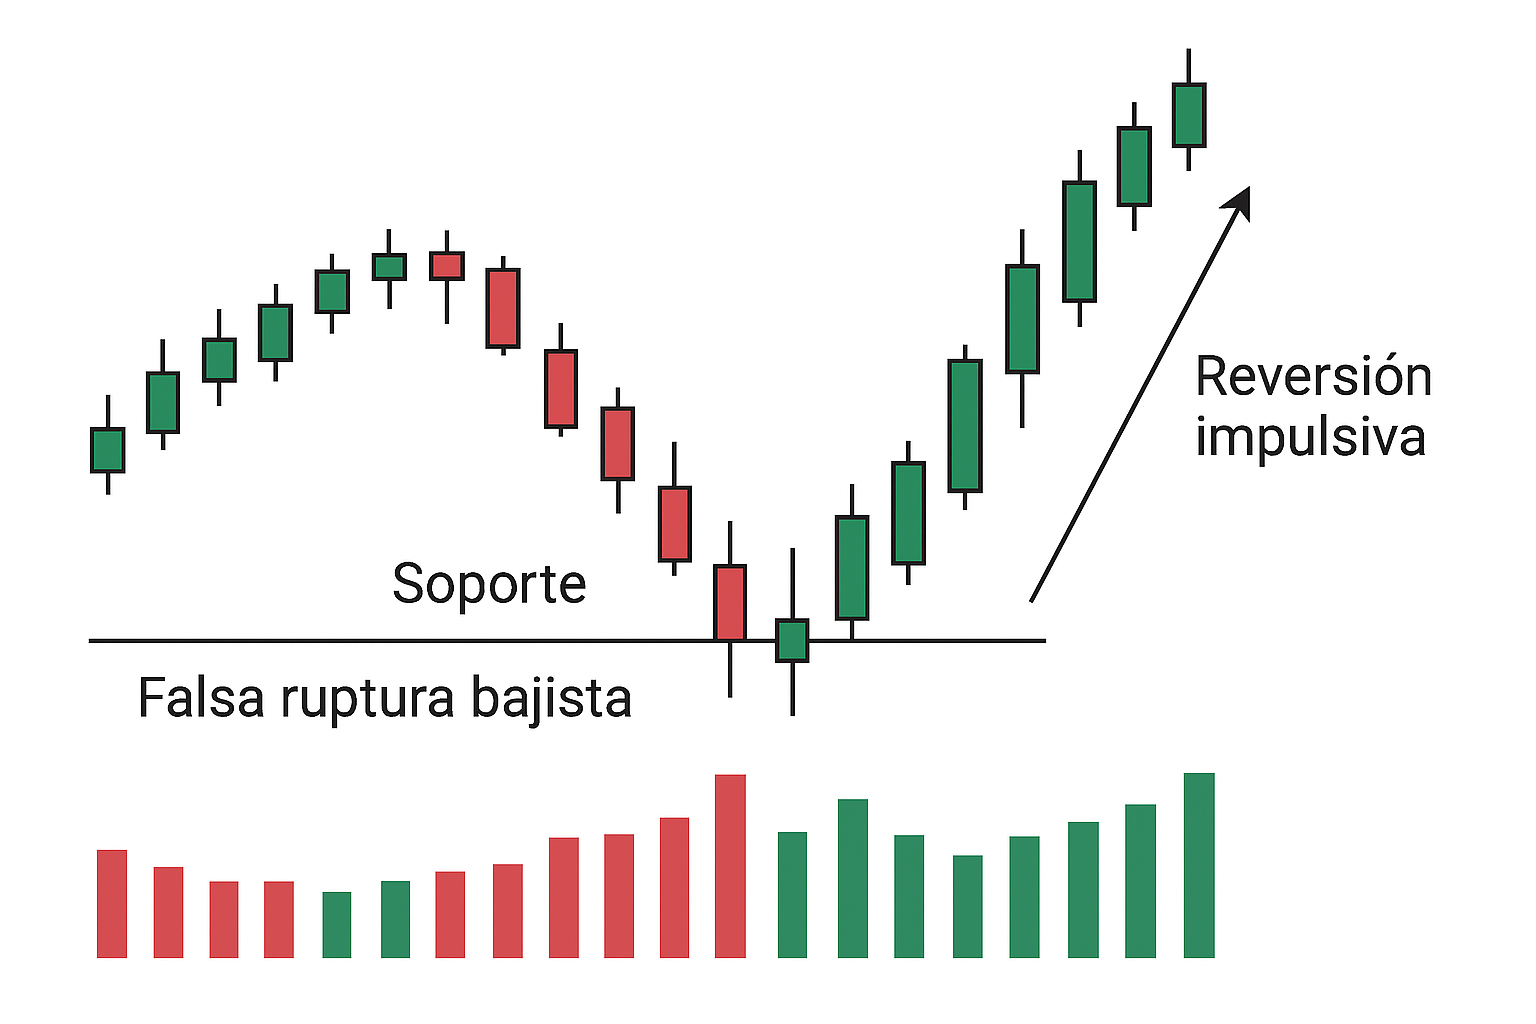
\includegraphics[width=11cm]{images/Dilatacion_Falsa_Ruptura.png}
    \caption{Falsa ruptura bajista seguida de reversi\'on impulsiva}
    \label{fig:Dilatacion_Falsa_Ruptura}
\end{figure}
\vspace{0.5em}

\noindent
En la figura \ref{fig:Dilatacion_Falsa_Ruptura} se ilustra un ejemplo cl\'asico de \textbf{dilataci\'on bajista}, tambi\'en denominada \textbf{falsa ruptura}, seguida por una \textbf{reversi\'on con intenci\'on}. Este tipo de estructura es descrita por \textbf{Miguel \'Angel Ram\'irez} como una maniobra de enga\~no profesional para capturar liquidez, y por \textbf{Al Brooks} como una ruptura fallida de un rango seguida de una entrada de segunda intenci\'on.

\begin{itemize}
    \item En la parte inferior del gr\'afico se destaca una \textbf{zona de soporte t\'ecnico}, la cual ha sido testeada previamente. Esta zona atrae atenci\'on por parte de operadores minoristas y algoritmos.

    \item La vela roja que rompe el soporte representa una \textbf{dilataci\'on}, caracterizada por su breve penetraci\'on del nivel sin continuidad posterior. El volumen es moderado o incluso bajo, y el precio no logra sostenerse por debajo del soporte.

    \item A continuaci\'on aparece una \textbf{vela verde de rechazo}, que anula la ruptura y confirma el fallo. Este es el punto de inflexi\'on que marca el \textbf{cambio de control institucional}.

    \item Lo que sigue es una \textbf{reversi\'on impulsiva}: varias velas alcistas consecutivas con cuerpo amplio, cierres en m\'aximos y volumen creciente. Esta secuencia confirma la intenci\'on institucional en direcci\'on contraria a la ruptura inicial.

    \item El patr\'on revela c\'omo el operador profesional induce al error a los traders menos experimentados, \textbf{absorbiendo su liquidez} antes de ejecutar el movimiento real.
\end{itemize}

\noindent
Este tipo de configuraci\'on es esencial dentro de la lectura institucional del mercado. Su correcta identificaci\'on permite al operador evitar trampas y alinearse con la verdadera intenci\'on del profesional, fortaleciendo la calidad de sus decisiones operativas.

\vspace{1em}
\noindent
\begin{figure}[!htbp]
    \centering
    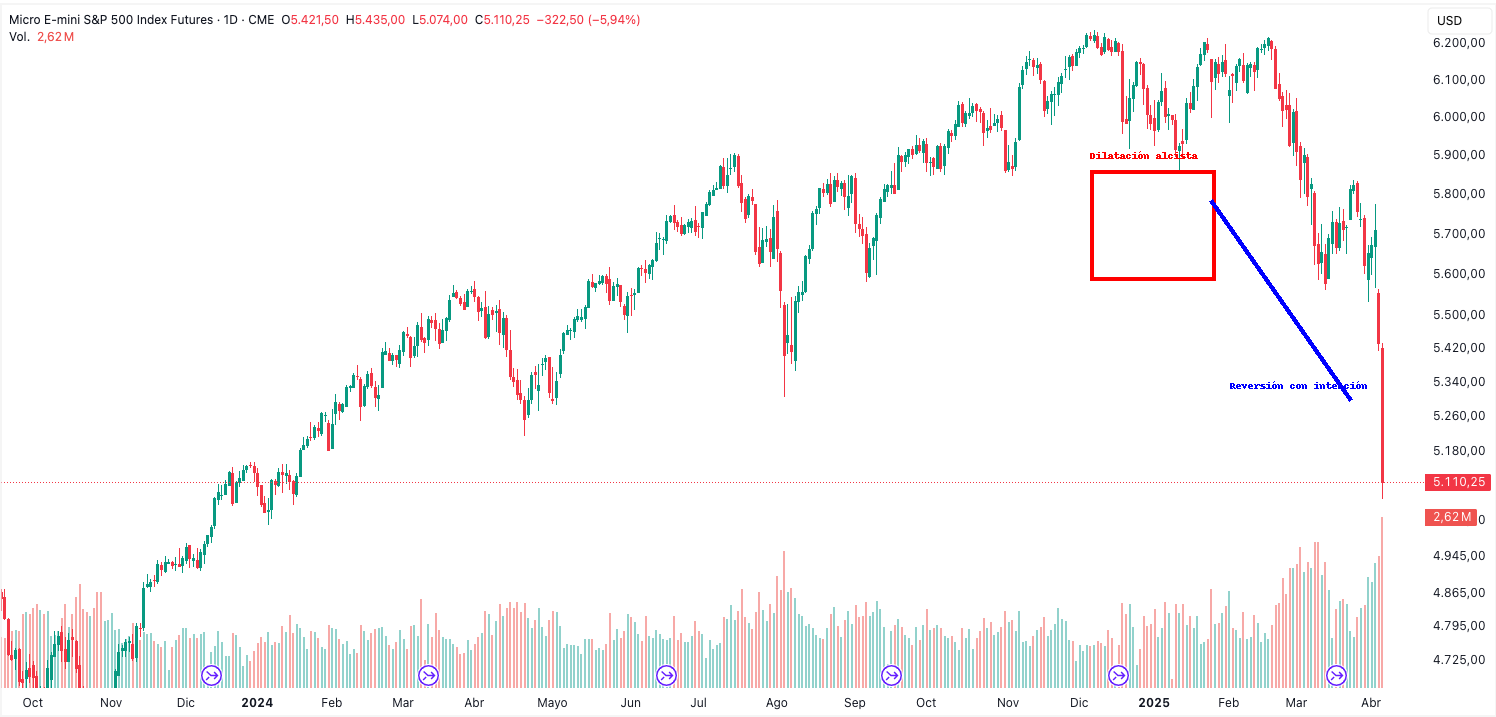
\includegraphics[width=11cm]{images/dilatacion_alcista_reversion.png}
    \caption{Dilataci\'on alcista en resistencia seguida de reversi\'on bajista con intenci\'on}
    \label{fig:dilatacion_alcista_reversion}
\end{figure}
\vspace{0.5em}

\noindent
La figura \ref{fig:dilatacion_alcista_reversion} muestra un caso representativo de \textbf{dilataci\'on alcista} o \textbf{falsa ruptura por encima de una resistencia relevante}, seguido por una \textbf{movilidad bajista con volumen e intenci\'on}, en el contrato MES-0625. Esta estructura es interpretada por \textbf{Miguel \'Angel Ram\'irez} como una trampa profesional orientada a inducir compras tard\'ias, y por \textbf{Al Brooks} como un fallo de ruptura que da paso a una entrada de segunda intenci\'on en sentido contrario.

\begin{itemize}
    \item La \textbf{zona roja} corresponde a una resistencia t\'ecnica previamente testeada por el precio. En dicha zona, el mercado rompe moment\'aneamente al alza, generando una aparente ruptura impulsiva que activa compras especulativas o stops de vendedores.

    \item Sin embargo, la ruptura carece de continuidad y es seguida por un \textbf{rechazo inmediato}, evidenciado en velas bajistas con volumen progresivamente mayor, lo que confirma la ausencia de convicci\'on institucional en la ruptura inicial.

    \item El movimiento posterior es una \textbf{reversi\'on bajista con intenci\'on}, en la que se suceden velas con cuerpo amplio, cierre en los extremos y volumen creciente. Esto valida el fallo como una maniobra de \textbf{distribuci\'on encubierta}.

    \item Esta dilataci\'on alcista permite redefinir el verdadero nivel de oferta institucional, y representa una oportunidad de entrada con ventaja informativa cuando se confirma el giro.
\end{itemize}

\noindent
Este tipo de secuencia es clave en la lectura profesional del mercado: permite identificar maniobras de manipulaci\'on por parte del operador institucional, y operar a favor del movimiento real con criterios de confirmaci\'on basados en \textbf{rechazo, volumen e intenci\'on}.


\subsection{Confirmaci\'on Operativa en Zonas Relevantes}

Para Brooks y Ram\'irez, la confirmaci\'on inmediata es clave para validar cualquier nivel relevante:

\begin{itemize}
    \item Una vela fuerte con volumen alto, seguida de continuidad en la direcci\'on de la ruptura, valida la zona relevante como punto de inflexi\'on genuino.
    
    \item La ausencia de continuidad posterior implica una falsa ruptura y ofrece una se\~nal operativa contraria, aprovechable por traders avanzados para incorporarse en sentido contrario al movimiento inicial enga\~noso.
\end{itemize}

\subsection{Integraci\'on Pr\'actica y Estrat\'egica}

Finalmente, una comprensi\'on profunda y operativa de estas zonas relevantes permite:

\begin{itemize}
    \item Detectar puntos cr\'iticos de entrada con riesgo controlado y alto potencial de recompensa.
    \item Reconocer tempranamente trampas profesionales y evitar posiciones desfavorables.
    \item Interpretar con claridad la intenci\'on profesional, tomando decisiones en consonancia con el verdadero flujo del mercado.
\end{itemize}

\subsection{Conclusi\'on sobre las Zonas Relevantes}

Las zonas relevantes, cuando se entienden profundamente desde el an\'alisis combinado del precio y volumen, ofrecen al operador una poderosa ventaja operativa. Ram\'irez y Brooks destacan la importancia de interpretar estas zonas desde la acci\'on real del mercado, reconociendo la intenci\'on profesional, validando las rupturas con volumen y buscando continuidad inmediata que confirme la fuerza real detr\'as de los movimientos. Este conocimiento profundo transforma la operativa en un ejercicio consciente y altamente efectivo, alineado con las fuerzas institucionales que realmente mueven los mercados.

\section{S\'intesis Operativa}

La combinaci\'on consciente de estos elementos convierte el trading en una pr\'actica profundamente profesional, alineada con las fuerzas institucionales dominantes, lo que aumenta significativamente las probabilidades de \'exito.

\begin{itemize}
    \item Identificaci\'on precisa de zonas relevantes.
    \item Confirmaci\'on de intenci\'on mediante testeo y secado.
    \item Interpretaci\'on de velas clave para entradas y salidas operativas.
    \item Gesti\'on estrat\'egica en contextos claramente definidos (dilataciones, recuperaciones, acumulaciones o distribuciones confirmadas).
\end{itemize}

``Encontrar la verdadera intenci\'on es la clave para poder actuar del lado correcto.''

\section*{Glosario t\'ecnico}

\vspace{1em}

\noindent A continuaci\'on se presenta un glosario operativo con las definiciones clave utilizadas en la estrategia, integrando terminolog\'ia de Ram\'irez, Brooks, Coulling y Neely:

\begin{description}[leftmargin=2cm, style=nextline]
    \item[Acumulaci\'on silenciosa:] Proceso de compras institucionales en una zona lateral con volumen bajo creciente y velas alcistas peque\~nas. Implica absorci\'on progresiva sin intenci\'on inmediata.
    
    \item[Distribuci\'on activa:] Zona de alto volumen con velas mixtas, donde grandes operadores venden posiciones en repuntes controlados. Suele finalizar con agotamiento.
    
    \item[Volumen de intenci\'on:] Volumen que excede el 2.5x del promedio en velas de rango medio-alto. Indica presencia institucional clara (Ram\'irez).
    
    \item[Stopping volume:] Pico de volumen en vela con sombra inferior prolongada y cierre en mitad o parte superior. Implica freno de ca\'ida y posible giro (Coulling).
    
    \item[Reversi\'on por pin bar:] Vela con mecha larga (superior o inferior), cuerpo peque\~no y volumen menor al promedio. Detecta trampas y rechazo institucional (Brooks).
    
    \item[Correcci\'on plana:] Estructura de 3 ondas ABC donde B sobrepasa el inicio de A y C no logra superar a A. Detecta consolidaci\'on inestable (Neely).
    
    \item[Zigzag correctivo:] Patr\'on impulsivo correctivo en 3 tramos (A–B–C) con retrocesos claros. Cierra estructura r\'apida de correcci\'on (Neely).
    
    \item[Divergencia volumen–precio:] Desfase entre aumento/disminuci\'on de precio sin confirmaci\'on del volumen. Se interpreta como se\~nal de agotamiento o trampa.
    
    \item[Canal alcista moderado:] Serie de m\'inimos y m\'aximos ascendentes con volumen constante o decreciente. Indica continuidad profesional sin euforia.
    
    \item[Rango estrecho:] Zona lateral con velas peque\~nas y volumen bajo. Suele preceder a movimiento brusco si hay absorci\'on acumulativa.
    
    \item[Trampa de ruptura:] Movimiento repentino fuera del rango con bajo volumen, seguido de retorno r\'apido. Indica enga\~no de mercado.
    
    \item[Testeo profesional:] Vela peque\~na tras un rally, con volumen bajo y sin seguimiento. Confirma absorci\'on o distribuci\'on previa.
    
    \item[Breakout v\'alido:] Ruptura con vela de cuerpo completo, volumen superior a 2.5x el promedio y sin mecha contraria dominante.
    
    \item[Backtest de nivel:] Regreso al nivel recientemente roto, con vela de rango medio y volumen decreciente. Valida continuidad.
    
    \item[Media direccional de 15m:] Media m\'ovil simple de 10 velas en marco de 15 minutos. Define sesgo institucional para filtrar entradas.
    
    \item[Engulfing decisivo:] Vela envolvente con cuerpo grande, que cubre al menos dos velas previas, con volumen 2x superior. Se\~nal fuerte de giro (Brooks).
\end{description}

\vspace{2em}

\subsection*{Ejemplos operativos por concepto}

A continuaci\'on se presentan ejemplos t\'ipicos de aplicaci\'on contextual en entorno real (nivel 5800, ES-0625):

\begin{itemize}
    \item \textbf{Acumulaci\'on silenciosa:} Zona entre 5790–5800 con velas alcistas peque\~nas y volumen estable (1800–2200 contratos), sin ruptura inmediata.
    
    \item \textbf{Stopping volume:} Vela con sombra inferior larga en 5788, cuerpo pequeño, volumen 5000 contratos; cierra en 5791. Implica absorci\'on institucional.
    
    \item \textbf{Trampa de ruptura:} Ruptura bajista de 5785 con volumen de 1000 contratos; siguiente vela engulfing alcista con 3500 contratos. Falsa ruptura detectada.
    
    \item \textbf{Correcci\'on plana irregular:} Estructura A: 5810–5790, B: 5790–5815, C: 5815–5805. Volumen decreciente en C y stopping volume en 5805.
\end{itemize}

\vspace{2em}

\subsection*{Ruido y trampas: detecci\'on y filtros operativos}

En marcos de 2 minutos, el ruido puede inducir entradas falsas o anticipadas. Para mitigar su impacto, se emplean los siguientes filtros:

\begin{itemize}
    \item \textbf{Filtro correctivo:} No operar dentro de estructuras correctivas activas (zigzag o plana) hasta confirmaci\'on de onda C con volumen e intenci\'on clara.

    \item \textbf{Filtro de divergencia:} Si el precio sube y el volumen decrece, evitar entradas alcistas. Confirmar con vela de agotamiento o rechazo (Coulling).

    \item \textbf{Filtro de validaci\'on institucional:} Si el volumen no alcanza el umbral din\'amico (2.2x media de 10 velas), no asumir ruptura ni continuidad.

    \item \textbf{Filtro de contexto multinivel:} Si la media de 15 minutos est\'a plana o en contra, abstenerse de operar. Esperar alineaci\'on.

    \item \textbf{Se\~nales de trampa comunes:}
    \begin{itemize}
        \item Vela pin bar con volumen bajo.
        \item Vela con cuerpo largo sin volumen.
        \item Doji tras vela impulsiva sin continuidad.
        \item Rango estrecho con volumen creciente.
    \end{itemize}
\end{itemize}
